\documentclass[11pt,a4paper]{article}
\usepackage[utf8]{inputenc}
\usepackage[margin=1in]{geometry}
\usepackage{lmodern}
\usepackage{microtype}
\usepackage{xcolor}
\usepackage{titlesec}
\usepackage{fancyhdr}
\usepackage{listings}
\usepackage{tcolorbox}
\usepackage{tikz}
\usetikzlibrary{shapes.geometric, arrows, positioning, fit, backgrounds}
\usepackage{hyperref}
\usepackage{amsmath}
\usepackage{amssymb}
\usepackage{booktabs}
\usepackage{graphicx}
\usepackage{float}
\usepackage{caption}
\usepackage{tabularx}

% Professional Color Palette
\definecolor{primary}{RGB}{30, 41, 59}    % Slate 800
\definecolor{secondary}{RGB}{71, 85, 105}  % Slate 600
\definecolor{accent}{RGB}{2, 132, 199}     % Sky 600
\definecolor{background}{RGB}{248, 250, 252} % Slate 50
\definecolor{border}{RGB}{226, 232, 240}     % Slate 200
\definecolor{safetyred}{RGB}{239, 68, 68}    % Red 500
\definecolor{confirmgreen}{RGB}{34, 197, 94} % Green 500

% Section Formatting
\titleformat{\section}{\Large\bfseries\color{primary}}{\thesection}{1em}{}[{\titlerule[0.5pt]}]
\titleformat{\subsection}{\large\bfseries\color{secondary}}{\thesubsection}{1em}{}
\titleformat{\subsubsection}{\normalsize\bfseries\color{primary}}{\thesubsubsection}{1em}{}

% Headers/Footers
\pagestyle{fancy}
\fancyhf{}
\fancyhead[L]{\small\color{secondary}Assignment 3: Agentic Shell (\texttt{doit})}
\fancyhead[R]{\small\color{secondary}Yuval Reuveni \& Arbel Tepper}
\fancyfoot[C]{\thepage}
\renewcommand{\headrulewidth}{0.4pt}
\renewcommand{\footrulewidth}{0pt}

% Hyperlink Configuration
\hypersetup{
    colorlinks=true,
    linkcolor=accent,
    citecolor=accent,
    urlcolor=accent,
    pdfauthor={Yuval Reuveni, Arbel Tepper},
    pdftitle={Assignment 3: Agentic Shell (doit) - Report}
}

% Code Listing Configuration
\lstset{
    backgroundcolor=\color{background},
    basicstyle=\ttfamily\small,
    breakatwhitespace=false,
    breaklines=true,
    captionpos=b,
    commentstyle=\color{secondary}\itshape,
    keywordstyle=\color{accent}\bfseries,
    numberstyle=\tiny\color{secondary},
    numbers=left,
    numbersep=8pt,
    showspaces=false,
    showstringspaces=false,
    showtabs=false,
    stringstyle=\color{teal},
    frame=single,
    rulecolor=\color{border},
    tabsize=2,
    escapeinside={(*@}{@*)},
    literate={—}{{---}}1 {–}{{--}}1 {‘}{{`}}1 {’}{{'}}1 {“}{{``}}1 {”}{{''}}1
}

% Custom TColorBox styles
\newtcolorbox{decisionbox}[1]{
    colback=background,
    colframe=secondary,
    coltitle=white,
    fonttitle=\bfseries\color{white},
    title=#1,
    arc=4pt,
    boxrule=1pt
}

\newtcolorbox{safetybox}[1]{
    colback=background,
    colframe=safetyred,
    coltitle=white,
    fonttitle=\bfseries\color{white},
    title=#1,
    arc=4pt,
    boxrule=1.5pt
}

\begin{document}

% TITLE PAGE
\begin{titlepage}
    \centering
    \vspace*{2cm}
    {\Huge\bfseries\color{primary} Assignment 3: Agentic Shell (\texttt{doit}) \par}
    \vspace{0.5cm}
    {\large\color{secondary} LLM-Class 2025-2026 \par}
    \vspace{1.5cm}
    
    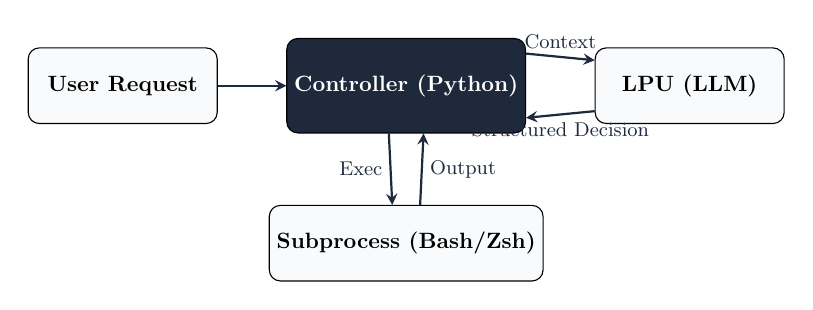
\begin{tikzpicture}[scale=0.8, every node/.style={transform shape}]
        % System Architecture Diagram in Title
        \node[draw, rectangle, fill=background, minimum width=3cm, minimum height=1.2cm, rounded corners] (user) at (0,0) {\bf User Request};
        \node[draw, rectangle, fill=primary, text=white, minimum width=3.5cm, minimum height=1.5cm, rounded corners] (ctrl) at (4.5,0) {\bf Controller (Python)};
        \node[draw, rectangle, fill=background, minimum width=3cm, minimum height=1.2cm, rounded corners] (lpu) at (9,0) {\bf LPU (LLM)};
        
        \draw[->, thick, >=stealth, color=primary] (user) -- (ctrl);
        \draw[->, thick, >=stealth, color=primary] (ctrl.15) -- node[above] {\small Context} (lpu.165);
        \draw[<-, thick, >=stealth, color=primary] (ctrl.345) -- node[below] {\small Structured Decision} (lpu.195);
        
        \node[draw, rectangle, fill=background, minimum width=3.5cm, minimum height=1.2cm, rounded corners] (shell) at (4.5,-2.5) {\bf Subprocess (Bash/Zsh)};
        \draw[->, thick, >=stealth, color=primary] (ctrl.250) -- node[left] {\small Exec} (shell.110);
        \draw[<-, thick, >=stealth, color=primary] (ctrl.290) -- node[right] {\small Output} (shell.70);
    \end{tikzpicture}
    
    \vspace{2.5cm}
    {\large\bfseries Authors: \par}
    {\large Yuval Reuveni \& Arbel Tepper \par}
    \vspace{1.5cm}
    
    \vfill
    {\large\color{secondary} July 2026 \par}
\end{titlepage}



% SECTION 2: SINGLE COMMAND AT A TIME
\section{Single command at a time.}
\label{sec:single_command}
The core requirement of this section is translating a single natural language request into a shell command, printing it, executing it in the user's active shell, and displaying the output.

\subsection{Implementation Details}
We developed the entry-point executable \texttt{doit} in Python (placed on the user's \texttt{PATH} via \texttt{\textasciitilde/.local/bin}). The system operates by assembling a system prompt, appending an environment block detailing the user's shell parameters, and calling the LPU with a command-step cap of \texttt{max\_steps=1}. 

If the user's prompt represents a command, the LPU calls the \texttt{run\_command} tool, which is intercepted and executed via Python's \texttt{subprocess.run}. If the prompt represents a general inquiry, the LPU responds with the \texttt{answer} tool.

\subsection{Design Decisions}

\begin{decisionbox}{Design Decision: Shell-Function Wrapper for Directory Navigation (\texttt{cd})}
    \textbf{Problem:} When a user runs a Python script, it runs in a child subprocess. Any directory change (\texttt{cd}) executed by the script is lost when the script exits, returning the user to the original terminal directory.
    
    \textbf{Solution:} We resolved this by writing a dual-shell wrapper. The \texttt{change\_dir} tool verifies that the path exists and writes it to a temporary file: \texttt{\textasciitilde/.doit/cd\_target\_\$DOIT\_SESSION}. Upon \texttt{doit}'s termination, a shell function wrapper intercepts the exit, checks for the presence of this file, runs the native \texttt{cd} command inside the parent shell, and deletes the file.
    \end{decisionbox}

\begin{decisionbox}{Design Decision: Dual-Shell Variable Normalization}
    \textbf{Context:} Since different team members use different operating systems and shells (e.g., macOS/Zsh vs. Linux/Bash), command arguments and behavior can diverge.
    
    \textbf{Solution:} The Controller auto-detects the host shell via \texttt{\$SHELL} and includes the shell type and operating system in the environment prompt block. The system prompt instructs the LPU to emit syntax tailored to the host environment.
\end{decisionbox}

\begin{decisionbox}{Design Decision: Primary API Model Selection}
    \textbf{Choice:} We selected \texttt{openai/gpt-4o-mini} as our primary API model. It is inexpensive, runs with low latency, and features robust native tool-calling capabilities that simplify core development.
\end{decisionbox}

\subsection{Example Interactions}
Below are two successful single-command interactions run using our primary model:

\begin{lstlisting}[language=bash, caption={Listing files including hidden ones.}]
$ doit "show me all files here, including hidden ones"
$ ls -la
total 232
drwxr-xr-x@  6 yuval  staff    192 Jul  7 18:23 acdl
-rw-r--r--@  1 yuval  staff  12405 Jul  7 18:24 CLAUDE.md
-rw-r--r--@  1 yuval  staff  30675 Jul  7 18:57 DECISIONS.md
-rwxr-xr-x@  1 yuval  staff   1319 Jul  7 15:00 doit
\end{lstlisting}

\begin{lstlisting}[language=bash, caption={Disk space command execution.}]
$ doit "how much disk space is left?"
$ df -h
Filesystem     Size   Used  Avail Capacity iused ifree %iused  Mounted on
/dev/disk3s1   926Gi   17Gi  702Gi     3%    459k  4.3G    0%   /
\end{lstlisting}

\subsection{ACDL Context Specification: DoitAgentSingleCommand}
The diagram below shows the context we build for a single-command turn: the system prompt, the environment block, and the user request. In single-command mode (\texttt{max\_steps=1}) the model makes one decision and the turn ends. The command's output is printed and logged, but it is never fed back to the model, so the diagram stops at the request.

\begin{figure}[H]
    \centering
    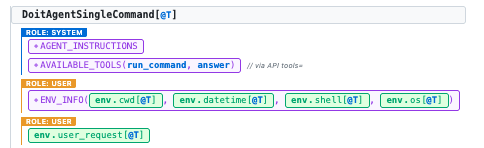
\includegraphics[width=0.9\textwidth]{acdl_v1.png}
    \caption{Visual representation of the ACDL context for DoitAgentSingleCommand.}
    \label{fig:acdl_v1}
\end{figure}

\lstinputlisting[numbers=none, basicstyle=\ttfamily\scriptsize, breaklines=true, caption={ACDL source for \texttt{DoitAgentSingleCommand} (\texttt{acdl/v1\_single.acdl}).}, label={lst:acdl_v1}]{../acdl/v1_single.acdl}

% SECTION 3: IDENTIFYING DANGEROUS COMMANDS
\section{Identifying dangerous commands}
\label{sec:safety}
To prevent the agent from accidentally corrupting the host machine or executing destructive actions without oversight, we implement safety policies that intercept filesystem mutations.

\subsection{Implementation Details}
Safety is handled through a double-layer verification policy (defense in depth):
\begin{enumerate}
    \item \textbf{LPU Self-Report (Layer 1):} The \texttt{run\_command} tool schema requires the LPU to populate the \texttt{is\_destructive} boolean flag and provide an \texttt{explanation} of what the command will do.
    \item \textbf{Deterministic Guard (Layer 2):} The Controller intercepts the decision and passes the command through a pre-compiled regex guard in \texttt{safety.py}. If the regex matches mutating operations (e.g. \texttt{rm}, \texttt{mv}, \texttt{cp}, \texttt{mkdir}, redirects \texttt{>}, \texttt{>>}, \texttt{git reset}), it overrides a false ``safe'' report, forcing \texttt{is\_destructive=True}.
\end{enumerate}

\subsection{Design Decisions}

\begin{decisionbox}{Design Decision: In-Band Self-Report vs. Separate LLM Judge Call}
    \textbf{Alternative Rejected:} We rejected using a separate LLM call to classify command destructiveness. 
    
    \textbf{Rationale:} A second LLM call doubles latency and API costs. Because the regex guard is required to handle safety deterministically anyway, we require the LPU to report destructiveness in the same JSON object as the command itself. The regex guard acts as the fallback mechanism. If the guard overrides the model's safety flag, the event is logged for analysis.
\end{decisionbox}

\begin{safetybox}{Safety Refusals vs. Confirmation Gates}
    \textbf{Hard Refusals:} Any command containing \texttt{sudo} or starting with an interactive full-screen program (e.g., \texttt{vim}, \texttt{nano}, \texttt{less}, \texttt{top}) is blocked immediately in the Controller. No confirmation is offered.
    
    \textbf{Confirmation Gates:} When a command is flagged destructive (either by the model or the regex override), the Controller halts, displays the command and its explanation, and prompts the user with \texttt{Proceed? [y/N]}. Execution only proceeds if the user inputs \texttt{y} or \texttt{yes}.
\end{safetybox}

\subsection{Example Interactions}

\begin{lstlisting}[language=bash, caption={Handling a destructive command with user confirmation.}]
$ doit "delete junk.txt"
[WARNING] This command modifies the filesystem:
    rm junk.txt
  This command deletes the file junk.txt.
Proceed? [y/N] y
$ rm junk.txt
\end{lstlisting}

\begin{lstlisting}[language=bash, caption={Interactive program refusal.}]
$ doit "open vim to write a story"
doit: 'vim' opens an interactive program doit can't wait for. Run it yourself:
    vim
\end{lstlisting}

\subsection{Guard Override in Practice}
The guard is not hypothetical. Across our 15 guard test cases it overrode the model's \texttt{is\_destructive} flag \textbf{6 times} (\texttt{logs/phase2/safety\_guard\_results.json}). A common case is a redirect that writes a file, which the model easily under-flags as read-only:

\begin{lstlisting}[language=bash, caption={A real guard override: the model reported the command as safe; the guard forced a confirmation.}]
command:              ls > files.txt
model is_destructive: false    (looks like a read-only listing)
guard is_destructive: true     (matched the ">" write-redirect pattern)
result:               Proceed? [y/N] gate shown before anything runs
\end{lstlisting}

\subsection{ACDL Context Specification: DoitAgentSafety}
The diagram below shows the only safety part the model actually sees: a \texttt{SAFETY\_INSTRUCTIONS} block in the system prompt. The regex guard and the \texttt{Proceed? [y/N]} gate run in Python and send nothing to the model, so they are not drawn. In short, the diagram shows what the model is told about safety, not how we enforce it.

\begin{figure}[H]
    \centering
    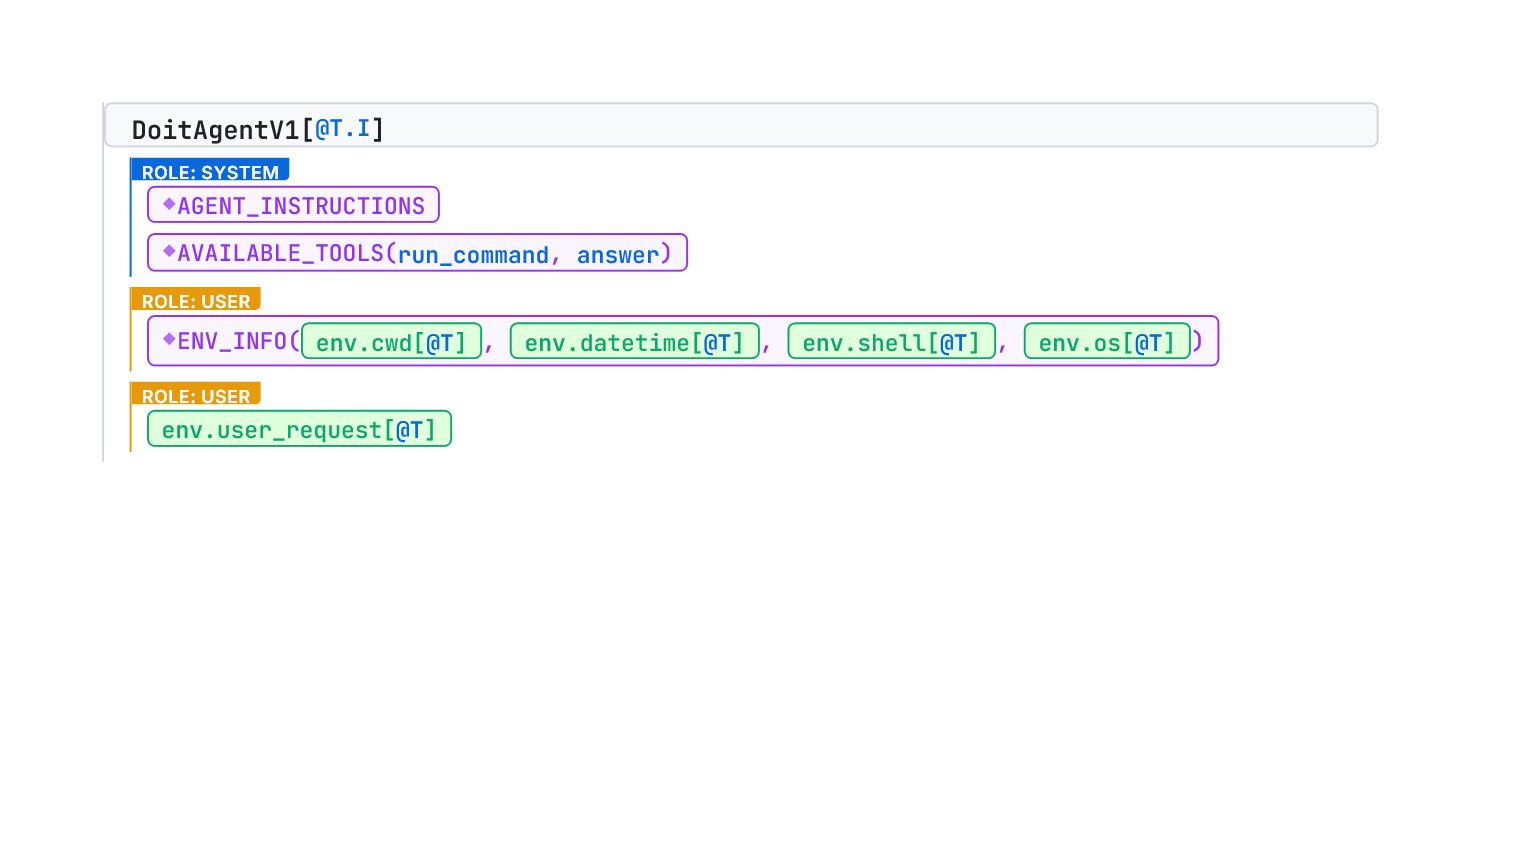
\includegraphics[width=0.9\textwidth]{acdl_v2.png}
    \caption{Visual representation of the ACDL context for DoitAgentSafety.}
    \label{fig:acdl_v2}
\end{figure}

\lstinputlisting[numbers=none, basicstyle=\ttfamily\scriptsize, breaklines=true, caption={ACDL source for \texttt{DoitAgentSafety} (\texttt{acdl/v2\_safety.acdl}).}, label={lst:acdl_v2}]{../acdl/v2_safety.acdl}

% SECTION 4: MODEL FLEXIBILITY
\section{Model flexibility}
\label{sec:model_flexibility}
To ensure the utility can run independently of commercial API keys, we extended the system to run local models locally.

\subsection{Implementation Details}
We introduced a configuration file \texttt{\textasciitilde/doit.cfg} to declare the active model and its adapter. We implement two code adapters behind a unified interface:

\begin{decisionbox}{Design Decision: Native vs. Prompted Adapter Architectures}
    \textbf{Native Adapter (\texttt{\_call\_native}):} For models supporting LiteLLM's JSON tool-calling protocol (e.g., \texttt{gpt-4o-mini}, \texttt{qwen3:4b-instruct}). LiteLLM passes tool schemas out-of-band and receives structured tool outputs.
    
    \textbf{Prompted Adapter (\texttt{\_call\_prompted}):} For local models that do not natively support tool-calling (e.g., \texttt{gemma3:4b}). It renders tool schemas as text, appends them to the system prompt, and enforces a strict JSON wrapper. To handle parser failures, we implement a string-based balanced brace scanner to locate JSON blocks, and allow \textbf{one retry} by appending the syntax error back to the LPU.
\end{decisionbox}

\subsection{Evaluation of Local Models}
We evaluated three models using the test suite in \texttt{tests/cases.md}:
\begin{table}[htbp]
    \centering
    \caption{Model capabilities and adapters.}
    \begin{tabularx}{\textwidth}{lllX}
        \toprule
        \textbf{Model Name} & \textbf{Deployment} & \textbf{Adapter} & \textbf{Tool-Calling Capability} \\
        \midrule
        \texttt{openai/gpt-4o-mini} & API (Remote) & Native & Full structured tool support \\
        \texttt{ollama/qwen3:4b-instruct} & Local (Ollama) & Native & Local tool-calling support \\
        \texttt{ollama/gemma3:4b} & Local (Ollama) & Prompted & None; relies on text JSON prompts \\
        \bottomrule
    \end{tabularx}
    \label{tab:models_eval}
\end{table}

\subsection{Analysis of Divergences and Failure Modes}

\subsubsection{Gemma-3 Impossible Request Failure}
When asked to perform a physically impossible command like \texttt{"make my laptop fly"}, the native models correctly responded with the conversational \texttt{answer} tool. However, the local \texttt{gemma3:4b} model (running under the prompted adapter) attempted to execute it via bash, choosing the \texttt{run\_command} tool with:
\begin{lstlisting}[language=bash]
echo "Sorry, I cannot make your laptop fly.""
\end{lstlisting}
Because the model appended a trailing double quote, the command crashed with a shell parse error: \texttt{zsh:1: unmatched "}.

\subsubsection{Prompted Adapter Recovery Logs}
Under the prompted adapter, local models often return markdown fences and conversational preambles. Below is a log showing our parser successfully stripping the preamble and recovering the JSON payload:
\begin{lstlisting}[caption={JSON de-fencing and brace-scanning recovery.}]
Raw LPU Output:
Sure, here is the command to view disk space:
```json
{
  "tool": "run_command",
  "args": {
    "command": "df -h",
    "is_destructive": false,
    "explanation": "Check available disk space."
  }
}
```
Parser Action: Strip fences, run brace scan -> extracted {"tool": "run_command", ...}
\end{lstlisting}

\subsection{Case-by-Case Results}
We ran cases 1--8 (basic) and 56--60 (hard single-command discriminators) from \texttt{tests/cases.md} on all three models in single-command mode (\texttt{enable\_plans=false}), so this is a clean translation test: one command per case, right or wrong. Table~\ref{tab:model_results} grades each turn.

\begin{table}[H]
    \centering
    \caption{Per-case results (V = correct command and outcome, $\sim$ = partial, X = wrong / failed / incorrectly refused).}
    \begin{tabular}{clccc}
        \toprule
        \# & Case & \texttt{gpt-4o-mini} & \texttt{qwen3:4b} & \texttt{gemma3:4b} \\
        \midrule
        1  & hidden files (\texttt{ls -a})      & V & X        & X \\
        2  & disk space (\texttt{df -h})        & V & V        & V \\
        3  & impossible request $\to$ refuse    & V & V        & X \\
        4  & joke $\to$ refuse                  & V & V        & V \\
        5  & ``how do I'' $\to$ answer          & V & X        & V \\
        6  & delete + confirm                   & V & V        & V \\
        7  & delete + abort                     & V & $\sim$   & V \\
        8  & redirect self-flag                 & V & V        & V \\
        56 & 5 largest, recursive, human-size   & V & X        & X \\
        57 & 3 most common words                & X & V        & X \\
        58 & non-blank \texttt{.py} lines       & X & X        & X \\
        59 & files modified $<$ 24h             & V & X        & X \\
        60 & rename \texttt{.txt} $\to$ \texttt{.md} & $\sim$ & V & X \\
        \midrule
        \multicolumn{2}{r}{\textbf{Correct count}} & \textbf{10} & \textbf{7} & \textbf{6} \\
        \bottomrule
    \end{tabular}
    \label{tab:model_results}
\end{table}

The ranking is \texttt{gpt-4o-mini} (10/13) $>$ \texttt{qwen3:4b} (7/13) $>$ \texttt{gemma3:4b} (6/13). Case 58 (count non-blank lines across nested \texttt{.py} files) is a good discriminator --- all three failed it. The clearest local-vs-local split is case 57 (3 most common words): \texttt{qwen3} produced the correct pipeline (\texttt{the}=4, \texttt{apple}=3, \texttt{fox}=2), while \texttt{gemma3} mis-flagged the read-only pipeline as destructive and aborted. On case 59 both local models emitted GNU-only \texttt{ls} flags (\texttt{--time-style}, \texttt{--block-size}) that fail on BSD/macOS, whereas \texttt{gpt-4o-mini} used a portable \texttt{find -mtime -1}.

\subsubsection{Logged Reliability Numbers}
\begin{itemize}
    \item The deterministic regex guard overrode the model's own \texttt{is\_destructive} flag in \textbf{6 of 15} guard test cases (\texttt{logs/phase2/safety\_guard\_results.json}); the same set also hard-blocked 1 \texttt{sudo} and 4 interactive commands.
    \item The prompted-adapter JSON parser passed \textbf{10/10} offline cases (\texttt{logs/phase3/prompted\_adapter\_results.json}), covering fenced JSON, JSON-in-prose, braces-inside-strings, hallucinated-tool rejection, and the retry path.
    \item Live, \texttt{qwen3} (native) produced \textbf{no} JSON/tool-call failures across all 13 cases; \texttt{gemma3} (prompted) hit one malformed reply it recovered from and one hard failure after two retries.
\end{itemize}

\subsection{ACDL Context Specification: DoitAgentPrompted}
For models without native tool-calling, tool schemas move into the system prompt prose, and the raw text reply is parsed. The visual ACDL diagram below shows how we handle JSON validation and retries:

\begin{figure}[H]
    \centering
    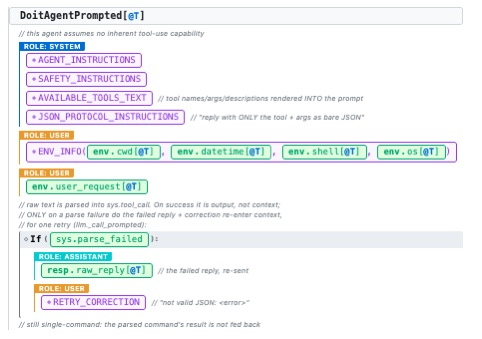
\includegraphics[width=0.9\textwidth]{acdl_v3.png}
    \caption{Visual representation of the ACDL context for DoitAgentPrompted.}
    \label{fig:acdl_v3}
\end{figure}

\lstinputlisting[numbers=none, basicstyle=\ttfamily\scriptsize, breaklines=true, caption={ACDL source for \texttt{DoitAgentPrompted} (\texttt{acdl/v3\_prompted.acdl}).}, label={lst:acdl_v3}]{../acdl/v3_prompted.acdl}

% SECTION 5: MULTI-TURN
\section{Multi-turn}
\label{sec:multi_turn}
To move from isolated commands to conversational sequences, we carry state across invocations, allowing commands to refer to previous outputs.

\subsection{Implementation Details}
When \texttt{doit} runs, it loads the session ID from the environment variable \texttt{DOIT\_SESSION} (which defaults to \texttt{"default"} if unset). The Controller reads and parses the JSONL session logs located at \texttt{\textasciitilde/.doit/sessions/\$DOIT\_SESSION.jsonl}, extracts the last $K=10$ turns, and splices them back into the prompt context.

\subsection{Design Decisions}

\begin{decisionbox}{Design Decision: JSONL Storage Format}
    \textbf{Problem:} Selecting an appropriate storage format for history.
    
    \textbf{Choice:} We chose JSONL (JSON Lines) files over SQLite. JSONL is lightweight, human-readable, and allows O(1) appends. It facilitates debugging and log evidence curation for the report.
\end{decisionbox}

\begin{decisionbox}{Design Decision: Tiered Truncation Budgets (\texttt{HOT} vs. \texttt{COLD})}
    \textbf{Problem:} Feeding complete command outputs (e.g. file listings or compiler logs) back into the prompt quickly overflows the context window.
    
    \textbf{Solution:} We implement a tiered head/tail truncation strategy. The active turn's output is allocated a \textbf{Hot Budget} (up to 3,000 characters head, 1,000 characters tail) to support follow-up decisions. Older replayed history turns are truncated to a \textbf{Cold Budget} (1,000 characters head, 300 characters tail), which provides enough context to resolve follow-ups (like referring to listed files) while saving tokens.
\end{decisionbox}

\subsection{Example Multi-Turn Interactions}
Below is a live multi-turn session log using \texttt{gpt-4o-mini}, demonstrating how the model changes flags and behavior rather than parroting commands:

\begin{lstlisting}[language=bash, caption={Relational multi-turn listing and sorting.}]
$ DOIT_SESSION=demo doit "list the files here"
$ ls -l
total 232
-rw-r--r--@  1 yuval  staff  12405 Jul  7 18:24 CLAUDE.md
-rw-r--r--@  1 yuval  staff  30675 Jul  7 18:57 DECISIONS.md

$ DOIT_SESSION=demo doit "now sort them by date"
$ ls -lt
total 232
-rw-r--r--@  1 yuval  staff  30675 Jul  7 18:57 DECISIONS.md
-rw-r--r--@  1 yuval  staff  12405 Jul  7 18:24 CLAUDE.md

$ DOIT_SESSION=demo doit "now in ascending order"
$ ls -ltr
total 232
-rw-r--r--@  1 yuval  staff  12405 Jul  7 18:24 CLAUDE.md
-rw-r--r--@  1 yuval  staff  30675 Jul  7 18:57 DECISIONS.md
\end{lstlisting}

\subsection{ACDL Context Specification: DoitAgentHistory}
The formal context structure representing the conversation history replay integration is detailed in the visual ACDL diagram below:

\begin{figure}[H]
    \centering
    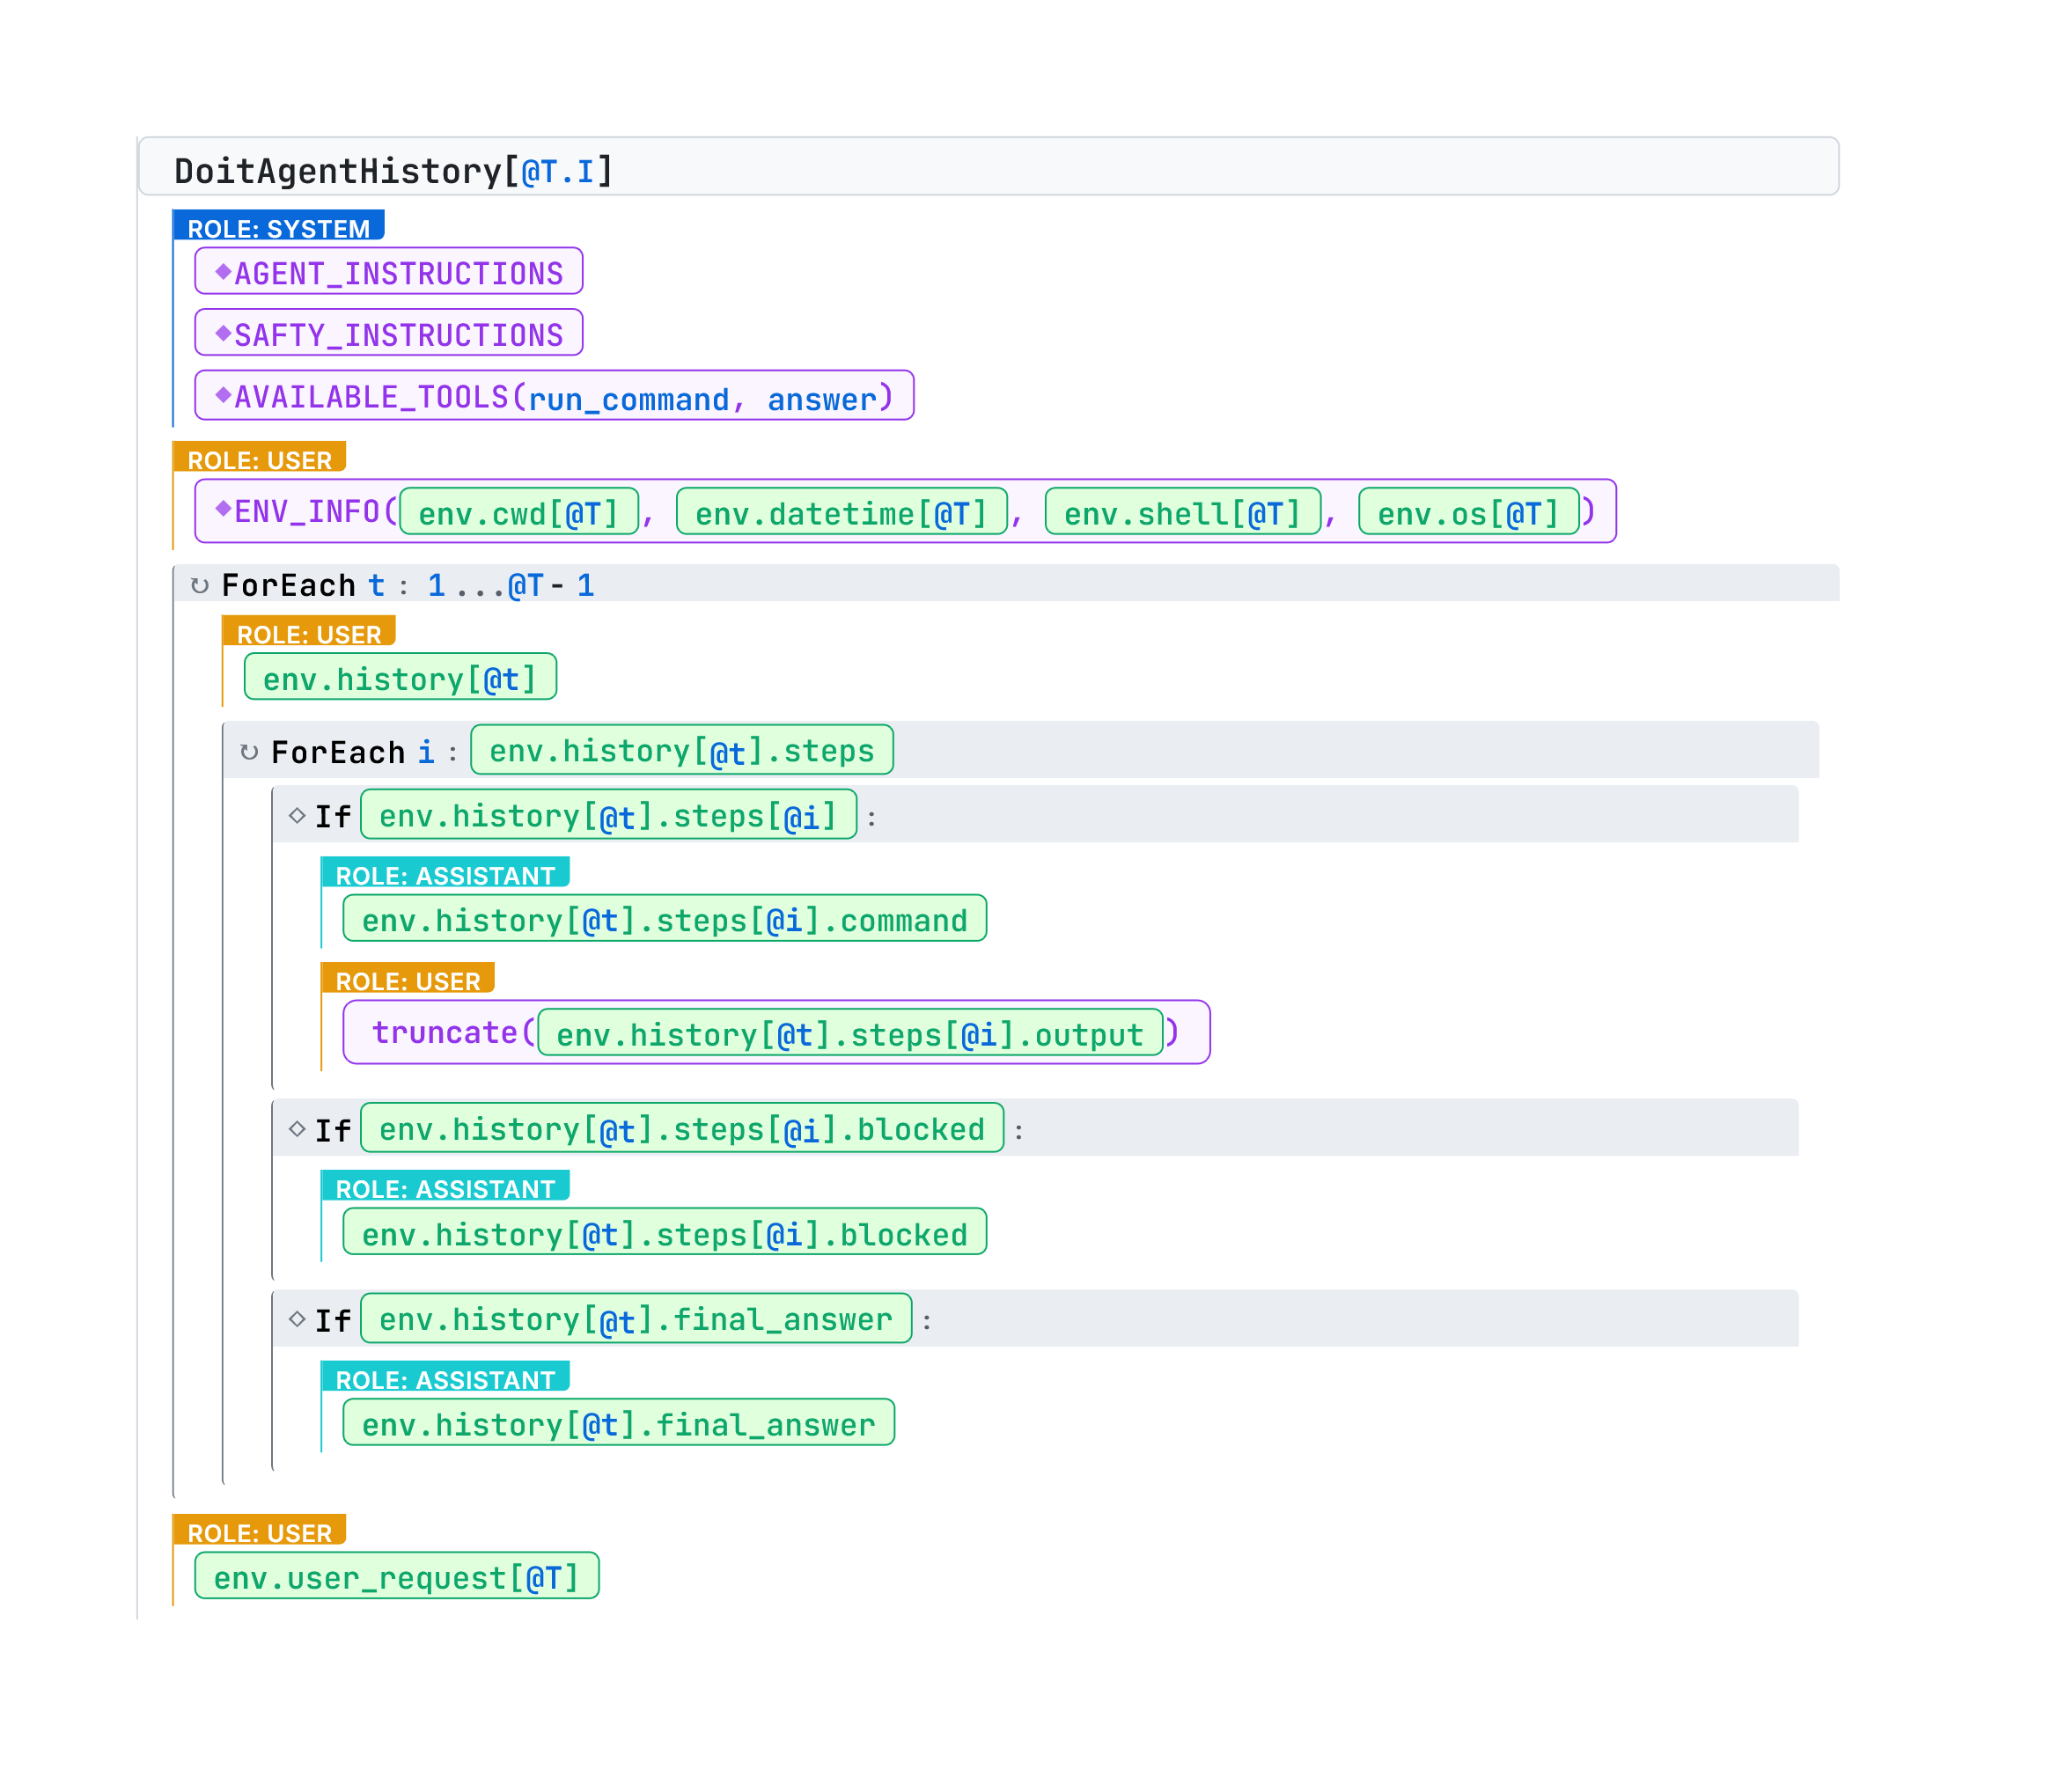
\includegraphics[width=0.9\textwidth]{acdl_v4.png}
    \caption{Visual representation of the ACDL context for DoitAgentHistory.}
    \label{fig:acdl_v4}
\end{figure}

\lstinputlisting[numbers=none, basicstyle=\ttfamily\scriptsize, breaklines=true, caption={ACDL source for \texttt{DoitAgentHistory} (\texttt{acdl/v4\_history.acdl}).}, label={lst:acdl_v4}]{../acdl/v4_history.acdl}

% SECTION 6: CLARIFICATIONS
\section{Clarifications}
\label{sec:clarifications}
When a user request is ambiguous, the agent must ask clarifying questions rather than guessing or executing a potentially harmful action.

\subsection{Implementation Details}
We introduce the \texttt{ask\_user} tool. When invoked by the LPU, the Controller prints the question alongside a numbered options menu, blocks on user input, and feeds the response back to the LPU. This process runs as a within-turn loop and does not count towards the command-step count.

\subsection{Design Decisions}

\begin{decisionbox}{Design Decision: Unanswered Clarification Default Behavior}
    \textbf{Problem:} How to proceed if the user presses Enter (empty input) or interrupts the prompt.
    
    \textbf{Solution:} Pressing Enter returns \texttt{"no answer"} to the LPU, instructing it to proceed with the default option it stated. If this default results in a destructive command, the Layer 2 safety confirmation gate (\texttt{Proceed? [y/N]}) still blocks execution. Pressing Ctrl-C raises a KeyboardInterrupt, aborts the turn immediately, and logs the abort status.
\end{decisionbox}

\subsection{Non-Annoyance Cap}
To prevent the agent from asking questions repeatedly, we implement two controls:
\begin{enumerate}
    \item \textbf{System Prompt Policy:} The LPU is instructed to ask questions only when a wrong guess is destructive, or when interpretations lead to different results with no clear default. Otherwise, it must assume the most common interpretation and state it in the final output.
    \item \textbf{Structural Cap:} We enforce a hard limit of \texttt{MAX\_CLARIFICATIONS=2} in the Controller. If the LPU exceeds this, the Controller feeds a capped message warning the model to commit to its best guess.
\end{enumerate}

\subsection{Example Interaction}
Below is a live interaction showing how the clarification loop and safety confirmation gate stack together cleanly:

\begin{lstlisting}[language=bash, caption={Stacked safety: clarification leading to a destructive confirmation gate.}]
$ doit "delete the logs"
Are you sure you want to delete the logs? This action cannot be undone.
  1. Yes
  2. No
Your answer (number or text): 1

[WARNING] This command modifies the filesystem:
    rm *.log
  This command deletes log files in the current directory.
Proceed? [y/N] y
$ rm *.log
\end{lstlisting}

\subsection{ACDL Context Specification: DoitAgentClarify}
The final formal context structure for our agent, representing both replayed turns and the within-turn clarification loop, is detailed in the visual ACDL diagram below:

\begin{figure}[H]
    \centering
    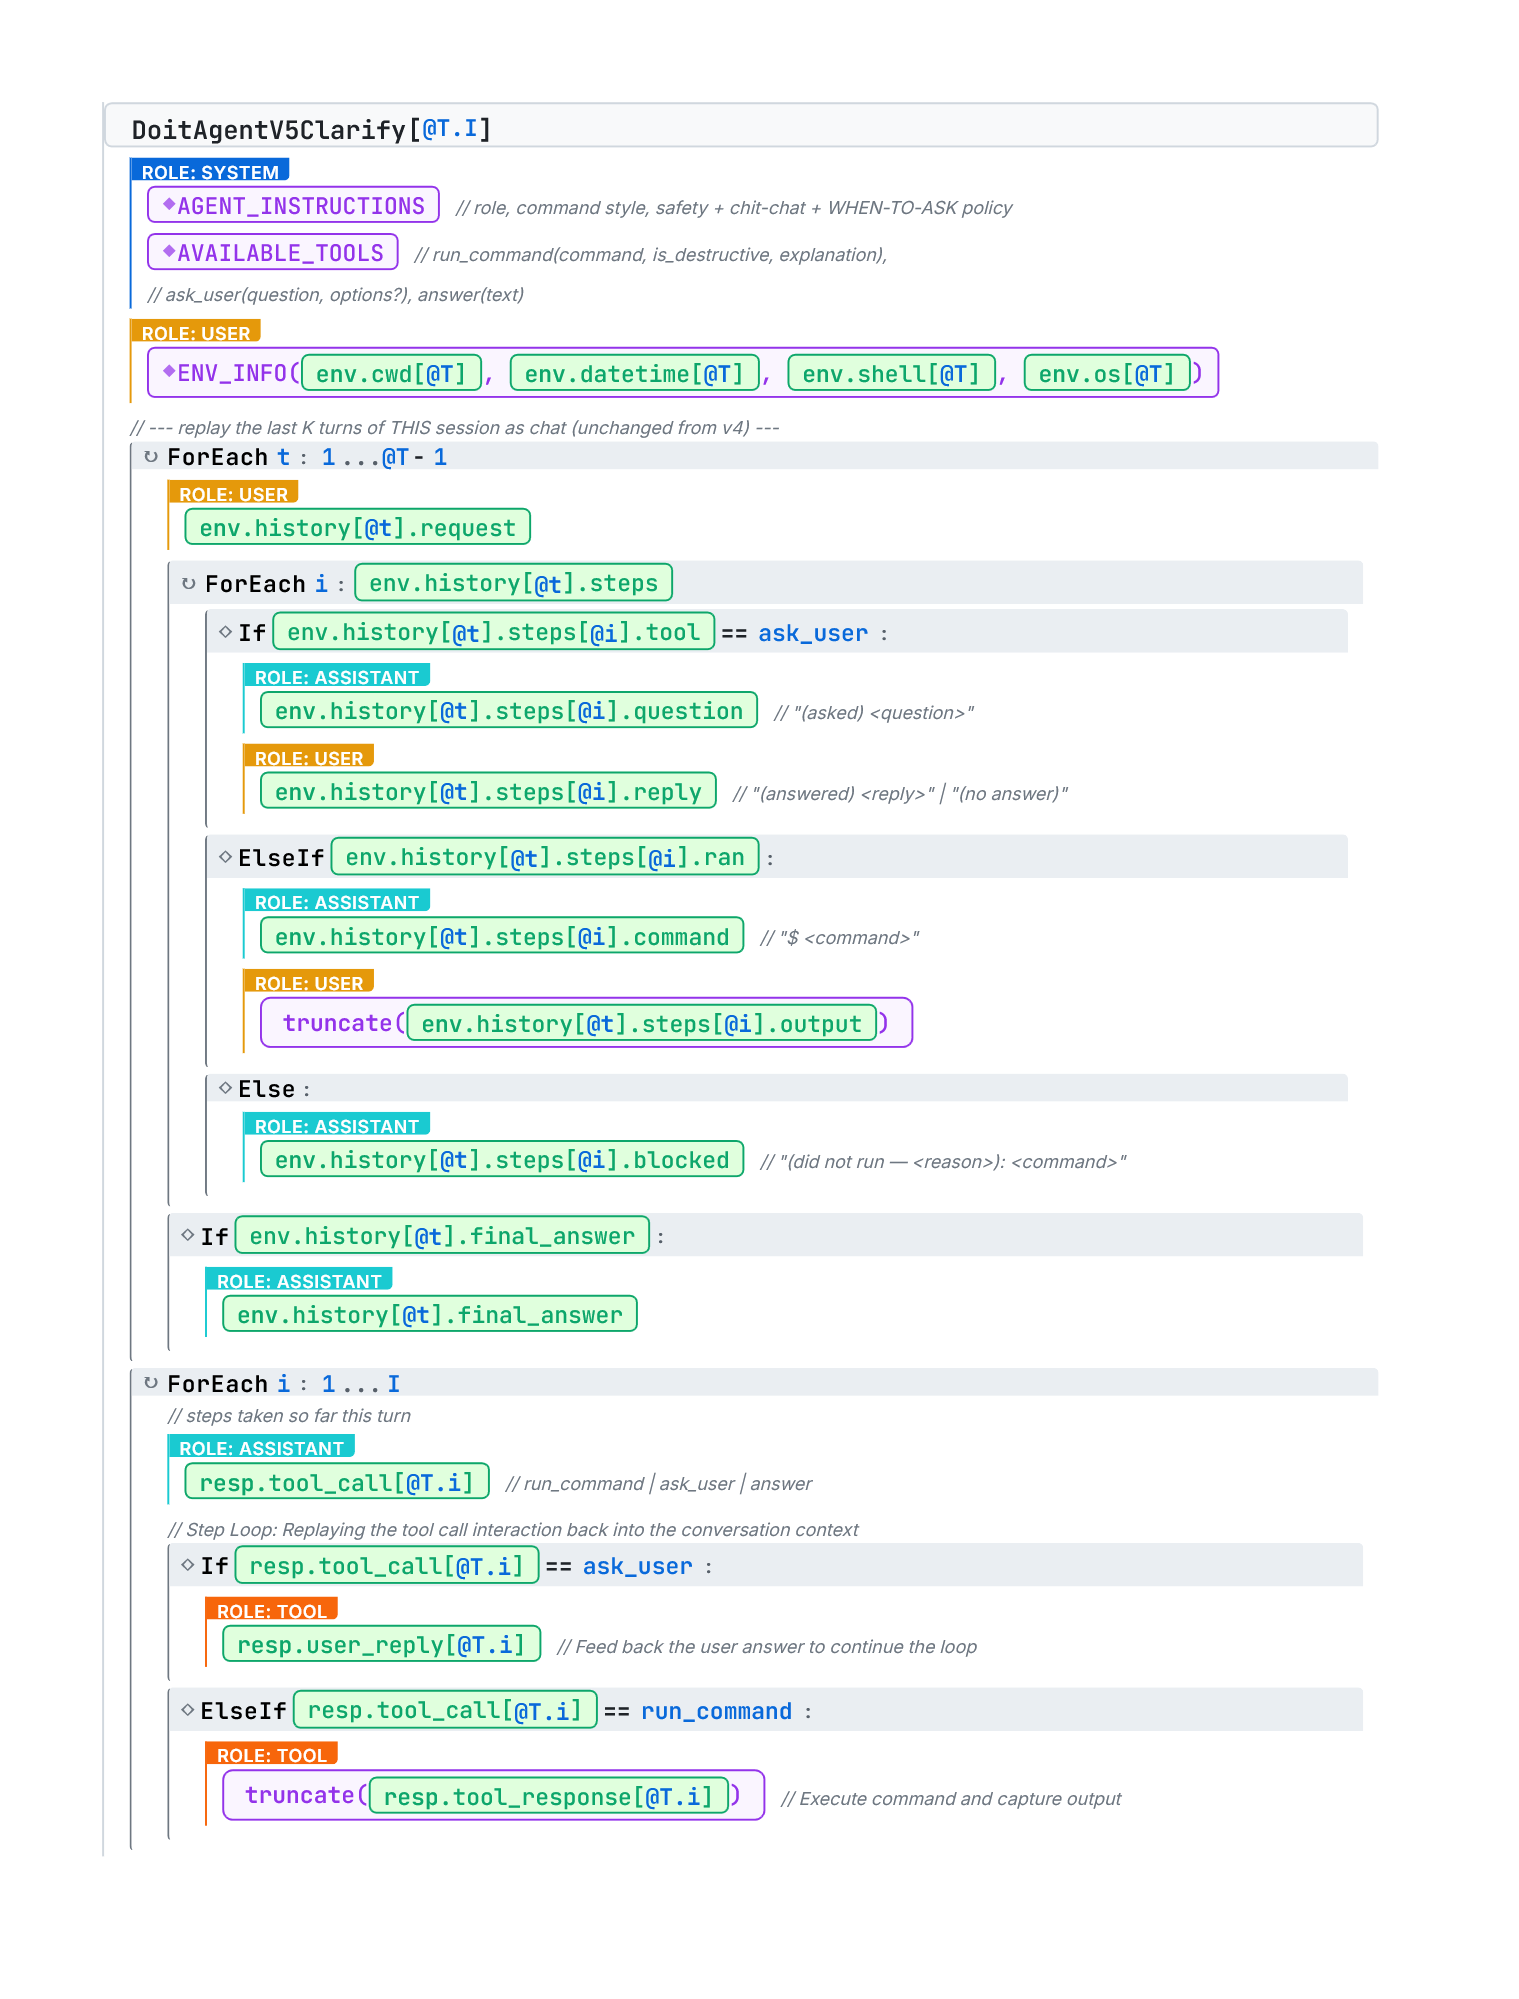
\includegraphics[width=0.9\textwidth]{acdl_v5.png}
    \caption{Visual representation of the ACDL context for DoitAgentClarify (clarifications and multi-turn history).}
    \label{fig:acdl_v5}
\end{figure}

\lstinputlisting[numbers=none, basicstyle=\ttfamily\scriptsize, breaklines=true, caption={ACDL source for \texttt{DoitAgentClarify} (\texttt{acdl/v5\_clarify.acdl}).}, label={lst:acdl_v5}]{../acdl/v5_clarify.acdl}

% SECTION 7: RICHER INTERACTIONS
\section{Richer interactions}
\label{sec:richer_interactions}
Richer interactions require the agent to respond to non-commands (e.g., ``how do I do X?'') and handle follow-up refinement chains (e.g., ``how do I list files?'' $\rightarrow$ ``modify it to show sizes'' $\rightarrow$ ``execute it'').

\subsection{Implementation Details}
We resolved this without introducing new tools or classification models. 
\begin{itemize}
    \item \textbf{Explaining vs. Running:} If a user asks a question, the LPU uses the \texttt{answer} tool. The Controller displays the answer and terminates the turn loop without executing commands.
    \item \textbf{Execution from History:} When the user subsequently requests ``execute it'', the request is sent with the session's turn history. The LPU reads the command structure it described in the previous \texttt{answer} and passes it to the \texttt{run\_command} tool.
\end{itemize}

\subsection{Example Interaction}
Below is a three-turn interaction chain showing history extraction and execution:
\begin{lstlisting}[language=bash, caption={How-do-I question, command modification, and execution.}]
$ doit "how do I find python files modified this week?"
You can use: find . -name "*.py" -mtime -7
$ doit "modify it to also show file sizes"
You can use: find . -name "*.py" -mtime -7 -ls
$ doit "execute it"
$ find . -name "*.py" -mtime -7 -ls
  14283    8 -rw-r--r--   1 yuval  staff  1319 Jul  7 15:00 ./doit
\end{lstlisting}

\subsection{Limitations}
We observed that smaller local models (such as \texttt{gemma3:4b}) frequently fail on the third turn (``execute it''), responding with ``Execute what?'' or hallucinating unrelated commands. This indicates that tracking command references across multiple conversational turns is a capability limited to larger, instruction-tuned models.

% SECTION 8: MEMORY
\section{Memory}
\label{sec:memory}
The memory subsystem allows the agent to persist long-term user facts across terminal windows, directories, and session boundaries.

\subsection{Implementation Details}
Memory storage is managed in \texttt{doitlib/state.py} via the flat JSON file \texttt{\textasciitilde/.doit/memories.json} (using the functions \texttt{load\_memories}, \texttt{add\_memory}, and \texttt{forget\_memory}). Unlike session history, this file is global and shared across all sessions. 

During context assembly, the controller invokes \texttt{memory\_block()} in \texttt{doitlib/context.py}, which formats the current memories using the template in \texttt{prompts/memory\_block.txt}. This block lists each stored fact with a short stable id (e.g., \texttt{m1}, \texttt{m2}) and injects them as \texttt{sys.memories}. This goes in its own \texttt{user} message, not the system prompt: only \texttt{agent\_instructions()} uses the \texttt{system} role, and every other block (memory included) is a \texttt{user} message.

The LPU manipulates these facts via two specialized tools: \texttt{remember(fact)} and \texttt{forget(id)}. Within the controller's turn loop, memory modifications are treated as within-turn steps. When the agent issues a memory tool call, the controller executes the state change in \texttt{\_handle\_memory} and immediately re-enters the execution loop (calling the LPU again) without decrementing the command step limit. This design allows the model to process memory changes and subsequently execute commands in a single user turn.

\subsection{Design Decisions}

\begin{decisionbox}{Design Decision: Global Shared Storage vs. Session-Keyed Memory}
    \textbf{Problem:} Determining the persistence scope for stored facts.
    
    \textbf{Alternative Rejected:} Storing memories inside the terminal's isolated session history.
    
    \textbf{Rationale:} Storing facts per session defeats the purpose of memory. If a user defines their project directory in one terminal, they expect that preference to be recognized when starting a fresh terminal or working in a different directory. Storing memories globally ensures they are visible across all terminal sessions.
\end{decisionbox}

\begin{decisionbox}{Design Decision: Memory Operations as Within-Turn Steps}
    \textbf{Problem:} Ensuring that metadata operations (like saving a fact) do not block or consume the execution budget.
    
    \textbf{Rationale:} If a user issues a command like \texttt{"remember this is my code folder and list files in it"}, the model must call \texttt{remember} followed by \texttt{run\_command}. If memory tool calls counted towards the command step budget (which defaults to 1), the agent would stop after memorizing, failing to execute the command. Processing memory tools as within-turn steps resolves this constraint.
\end{decisionbox}

\subsection{Example Interaction}
Below is a multi-session interaction where a memory saved in one terminal window is retrieved in another:

\begin{lstlisting}[language=bash, caption={Memory storage and cross-session retrieval.}]
Terminal A:
$ doit "remember that ~/school/llms/ass3 is my LLM class project folder"
Fact stored.

Terminal B:
$ doit "go to my LLM class project folder"
$ change_dir ~/school/llms/ass3
\end{lstlisting}

\subsection{Limitations}
\begin{decisionbox}{Design Decision/Limitation: Monotonic ID Generation and Reuse}
    \textbf{Behavior:} Memory IDs are generated dynamically as \texttt{m\{max\_id + 1\}}. If the highest ID is forgotten, its identifier is recycled for the next memory addition.
    
    \textbf{Limitation:} While this keeps identifiers short and readable, it creates a potential reference conflict in long-term history records. If an old replayed turn references a recycled ID, the context might contain a different fact than what the model originally saw. We accepted this limitation due to the small scale of memories (typically under a dozen facts).
\end{decisionbox}

\subsection{ACDL Context Specification: DoitAgentMemory}
The context structure representing the persistent memory block injection is detailed in the visual ACDL diagram below:

\begin{figure}[H]
    \centering
    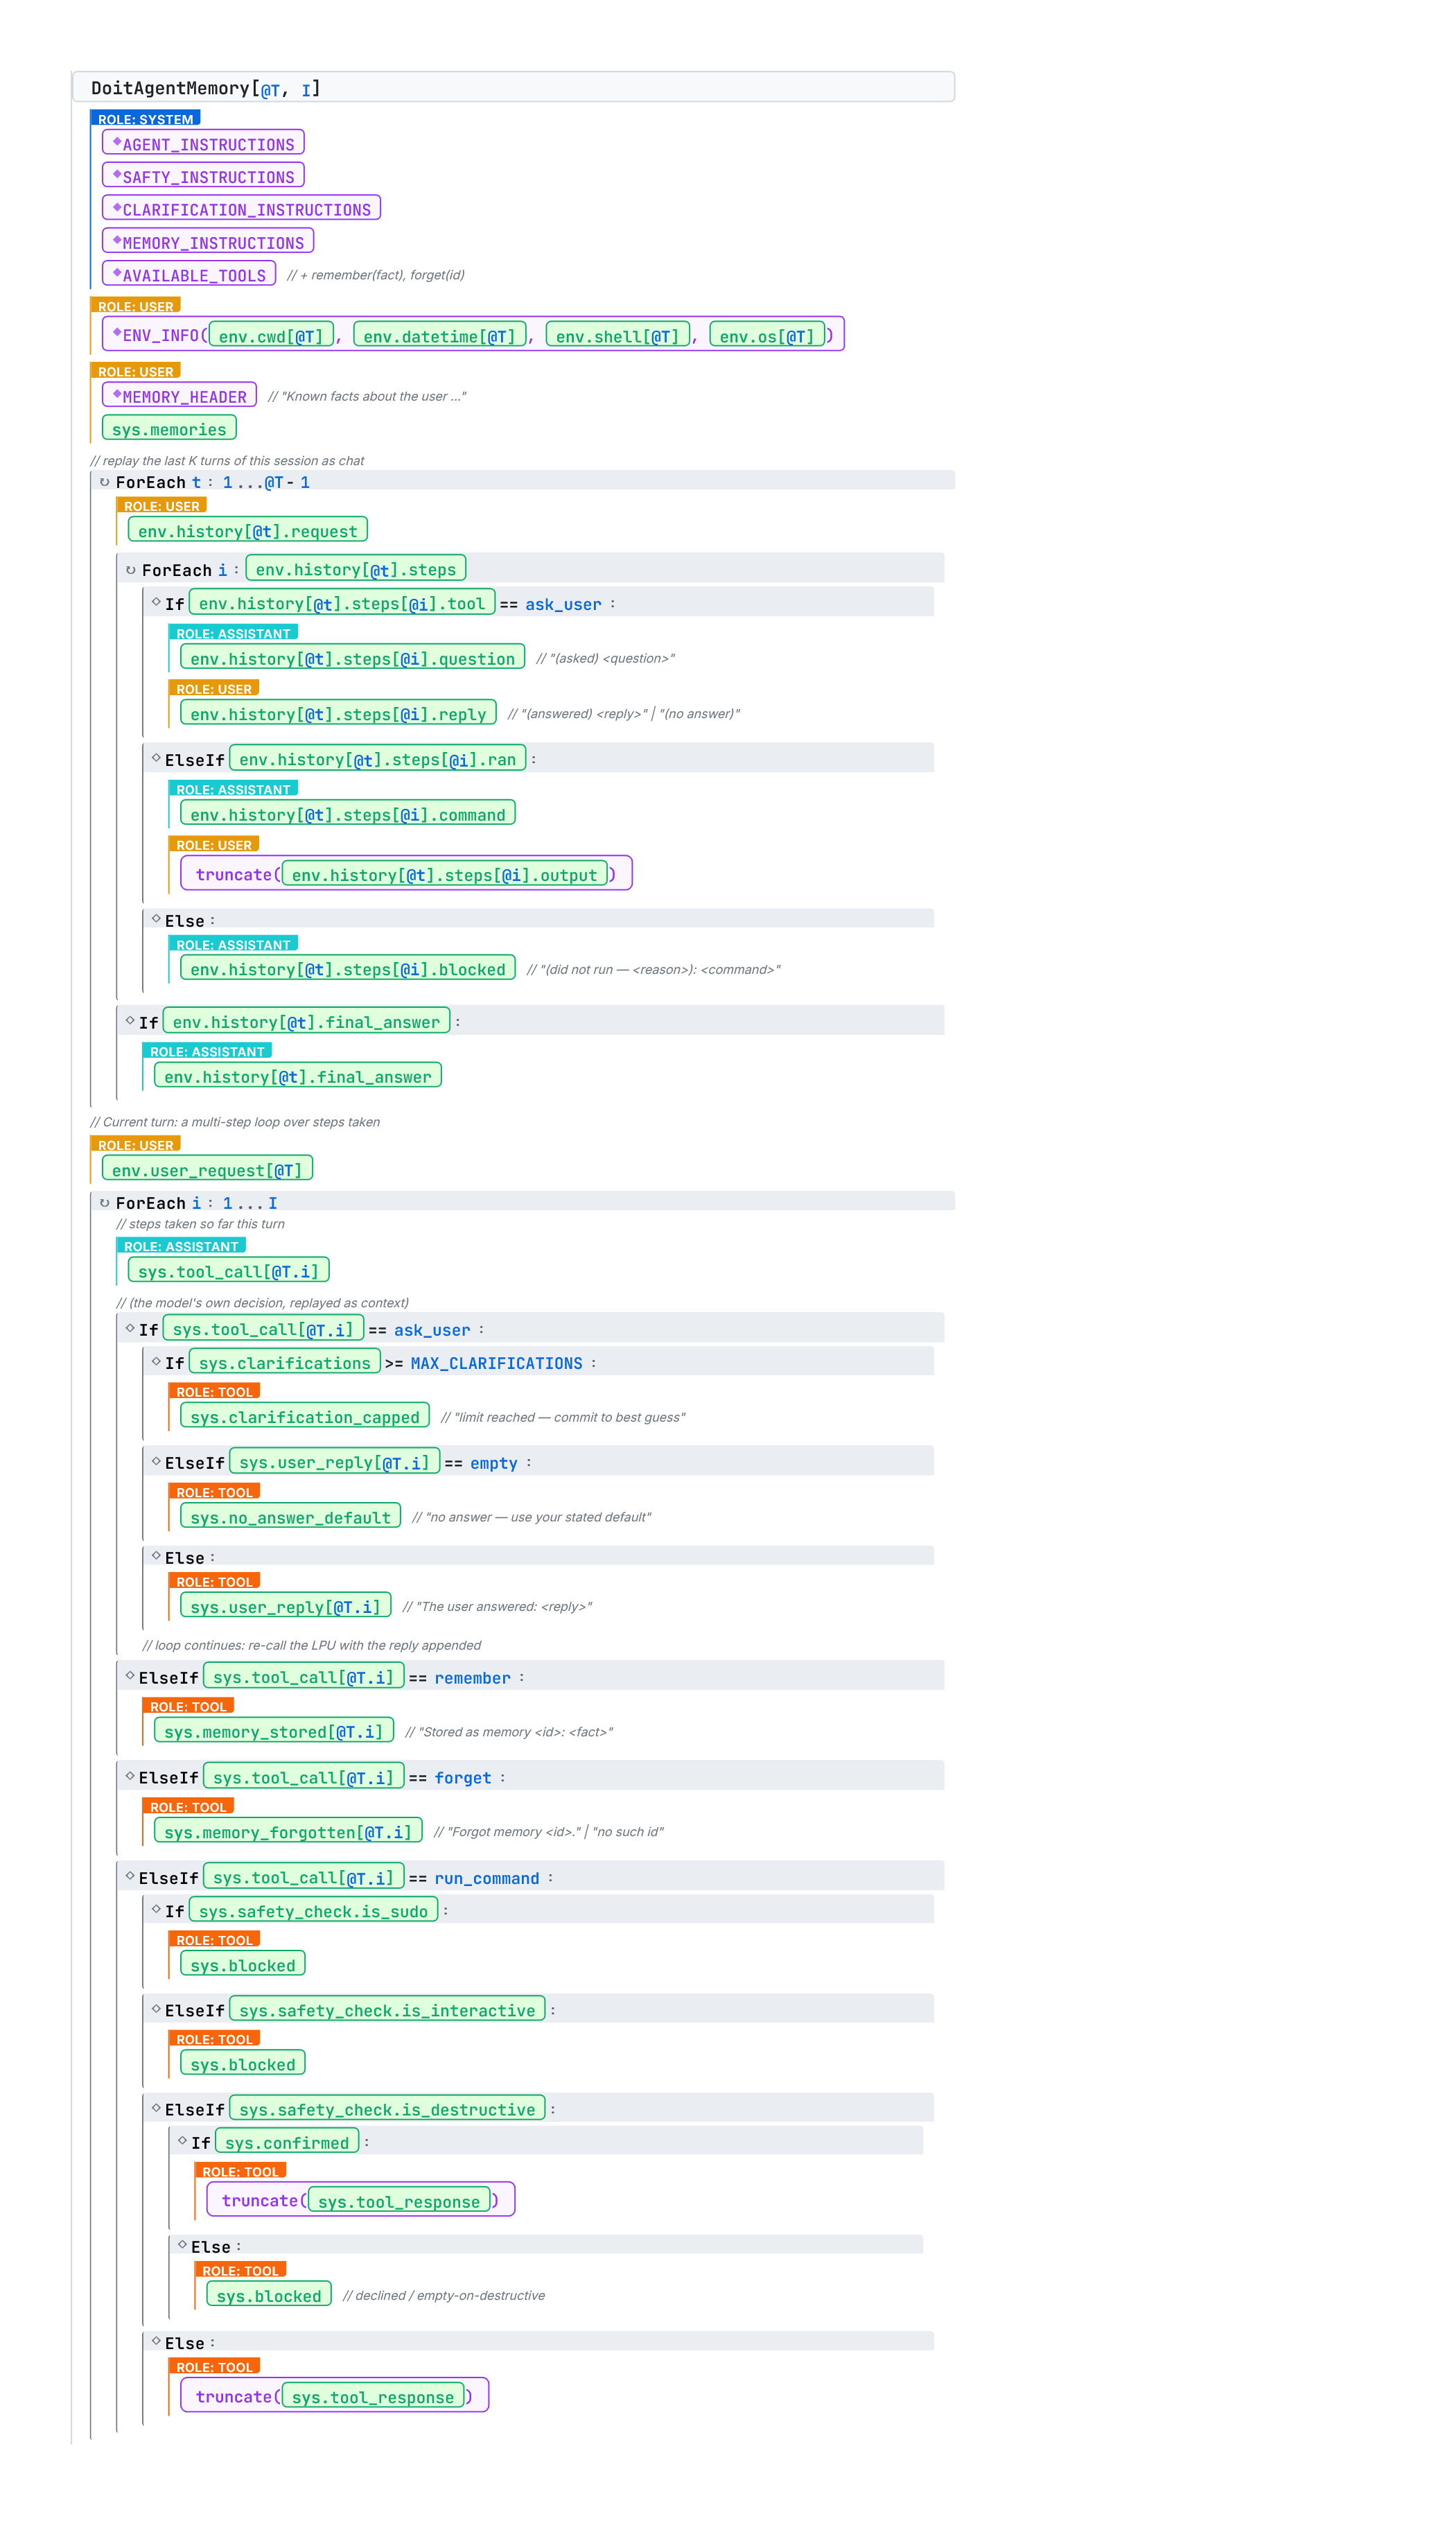
\includegraphics[width=0.9\textwidth]{acdl_v6.png}
    \caption{Visual representation of the ACDL context for memory injection.}
    \label{fig:acdl_v6}
\end{figure}

\lstinputlisting[numbers=none, basicstyle=\ttfamily\scriptsize, breaklines=true, caption={ACDL source for \texttt{DoitAgentMemory} (\texttt{acdl/v6\_memory.acdl}).}, label={lst:acdl_v6}]{../acdl/v6_memory.acdl}

% SECTION 8.5: CHANGE_DIR
\section{Changing directories (\texttt{change\_dir})}
\label{sec:change_dir}
Before adding user awareness, we fixed the \texttt{cd} trap (see the wrapper decision in Section~\ref{sec:single_command}). A Python subprocess cannot change its parent shell's directory, so we added a \texttt{change\_dir(path)} tool. It checks that the path exists and writes it to \texttt{\textasciitilde/.doit/cd\_target\_\$DOIT\_SESSION}; the shell wrapper reads that file after \texttt{doit} exits and runs the real \texttt{cd}. Like \texttt{remember}/\texttt{forget}, it is a within-turn step, so ``go there and list it'' can call \texttt{change\_dir} and then \texttt{run\_command} in the same turn.

One catch we found while testing: a \texttt{run\_command} in the same turn still runs in the \emph{old} directory, because the real \texttt{cd} only happens after the process exits. So the model has to point a same-turn command at the resolved path. The path check and the file write are Controller/shell work, so the diagram only shows the one result string the model gets back.

\begin{figure}[H]
    \centering
    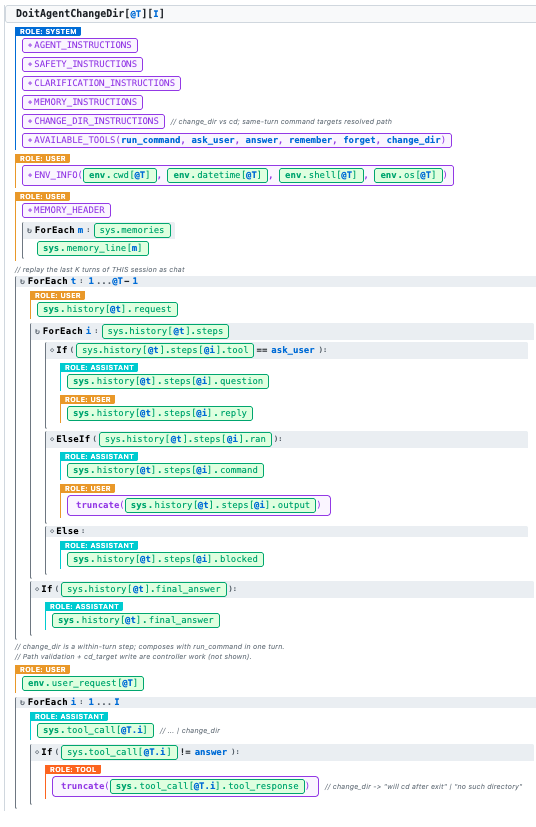
\includegraphics[width=0.9\textwidth]{acdl_v6-5.png}
    \caption{Visual representation of the ACDL context for DoitAgentChangeDir.}
    \label{fig:acdl_v6_5}
\end{figure}

\lstinputlisting[numbers=none, basicstyle=\ttfamily\scriptsize, breaklines=true, caption={ACDL source for \texttt{DoitAgentChangeDir} (\texttt{acdl/v6\_5\_changedir.acdl}).}, label={lst:acdl_v6_5}]{../acdl/v6_5_changedir.acdl}

% SECTION 9: USER AWARENESS
\section{User awareness}
\label{sec:user_awareness}
To enhance agent comprehension of manual shell actions, we capture the user's manual terminal command history and inject it into the agent's context.

\subsection{Implementation Details}
Shell integration snippets (appended to \texttt{\textasciitilde/.zshrc} or \texttt{\textasciitilde/.bashrc}) define a shell hook (\texttt{precmd} in Zsh, \texttt{PROMPT\_COMMAND} in Bash) that automatically writes every shell command executed by the user to a per-session log file: \texttt{\textasciitilde/.doit/shell\_hist/\$DOIT\_SESSION} in the format \texttt{timestamp|cwd|command}.

When \texttt{doit} runs, the controller calls \texttt{load\_recent\_user\_commands} in \texttt{doitlib/state.py}. This helper reads the raw shell history and filters out commands starting with the word \texttt{doit} to isolate manual user actions. The controller then compiles the last 20 filtered commands using \texttt{user\_shell\_history\_block} in \texttt{doitlib/context.py} (following the template in \texttt{prompts/user\_shell\_history\_block.txt}) and appends them to the context as a list of manual command entries.

\subsection{Design Decisions}

\begin{decisionbox}{Design Decision: Python-Side Log Filtering vs. Shell Hook Filtering}
    \textbf{Alternative Rejected:} Filtering out \texttt{doit} invocations inside the shell configuration hook itself.
    
    \textbf{Rationale:} Shell-side configurations are fragile and can easily crash prompt drawing or command resolution if they hit syntax errors. We chose to log all commands indiscriminately from the shell, delegating the filtering and parsing logic to Python where it can be managed safely.
\end{decisionbox}

\begin{decisionbox}{Design Decision: Isolated Per-Terminal History Streams}
    \textbf{Rationale:} Logging command history under a session-keyed folder \texttt{shell\_hist/\$DOIT\_SESSION} guarantees that manual actions typed in Terminal A do not pollute Terminal B's context, maintaining local alignment.
\end{decisionbox}

\subsection{Example Interaction}
Below is a live session where the agent retrieves and explains a manual command failure:

\begin{lstlisting}[language=bash, caption={Retrieving manual history to explain command failure.}]
$ mkdir reports
$ cd reports
$ cat status.log
cat: status.log: No such file or directory
$ doit "why did my last command fail?"
The command 'cat status.log' failed because there is no file named 'status.log' inside the 'reports' folder you just created.
\end{lstlisting}

\subsection{Limitations}
\begin{decisionbox}{Design Decision/Limitation: Manual Dotfile Synchronization}
    \textbf{Problem:} Updates to the snippet template in \texttt{shell/zshrc\_snippet.sh} do not automatically synchronize with the user's active configuration file.
    
    \textbf{Limitation:} If the shell hooks change in the codebase, the user must manually re-copy and re-source the snippet. Automating this sync was rejected to avoid corrupting dotfiles.
\end{decisionbox}

\subsection{ACDL Context Specification: DoitAgentUserAware}
The context structure representing manual user shell history injection is detailed in the visual ACDL diagram below:

\begin{figure}[H]
    \centering
    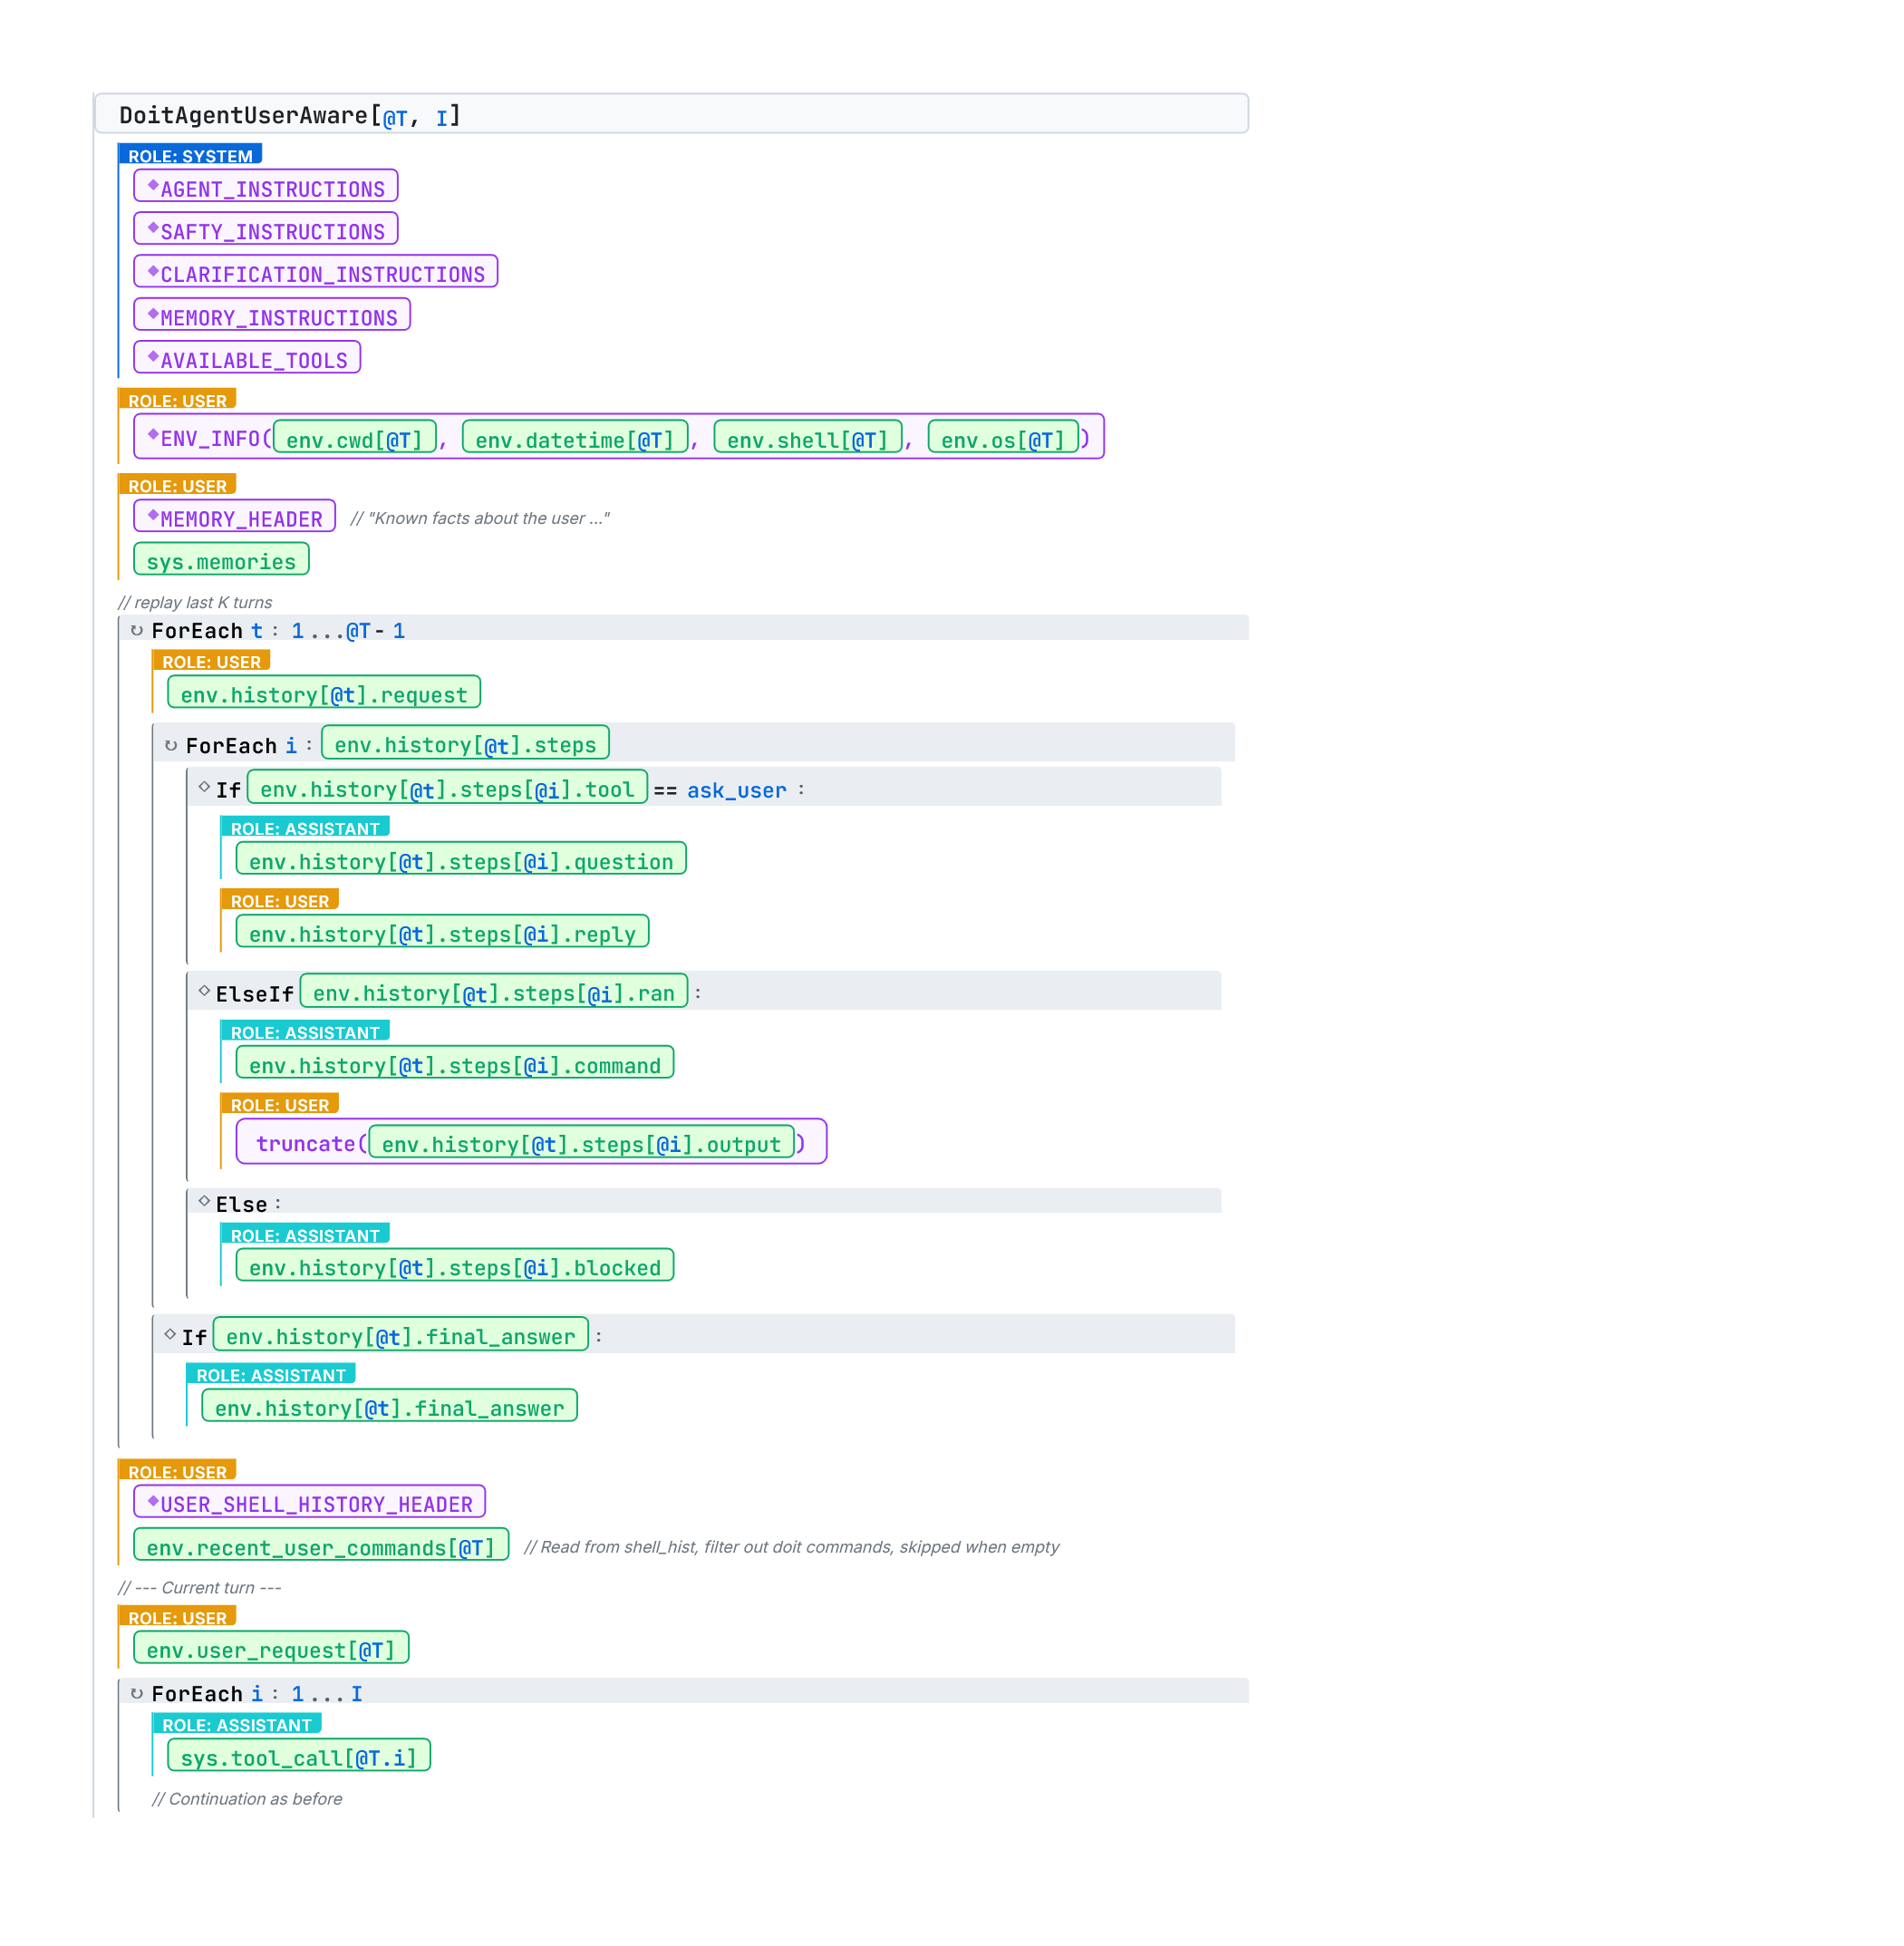
\includegraphics[width=0.9\textwidth]{acdl_v7.png}
    \caption{Visual representation of the ACDL context for user shell history awareness.}
    \label{fig:acdl_v7}
\end{figure}

\lstinputlisting[numbers=none, basicstyle=\ttfamily\scriptsize, breaklines=true, caption={ACDL source for \texttt{DoitAgentUserAware} (\texttt{acdl/v7\_useraware.acdl}).}, label={lst:acdl_v7}]{../acdl/v7_useraware.acdl}

% SECTION 10: OUTPUT AWARENESS
\section{Output awareness}
\label{sec:output_awareness}
To satisfy output-awareness requirements, the agent must be able to inspect previous command execution stdout, stderr, and return codes to answer follow-up queries.

\subsection{Implementation Details}
When \texttt{run\_command} executes a shell instruction, the controller captures the return code, stdout, and stderr. These outputs are stored inside the session history JSONL logs.

When building the context for subsequent turns, the controller replays the past turns. To prevent token bloat, the controller applies a tiered truncation strategy defined in \texttt{doitlib/tools.py} via \texttt{truncate\_for\_context(text)}:
\begin{itemize}
    \item \textbf{Hot Budget:} The output of the current/most-recent turn is allocated up to 3,000 characters head and 1,000 characters tail, ensuring listings and detailed compiler outputs are fully accessible.
    \item \textbf{Cold Budget:} Older turns in the history are truncated to 1,000 characters head and 300 characters tail, which is sufficient to capture errors or file lists without exceeding context limits.
\end{itemize}

\subsection{Design Decisions}

\begin{decisionbox}{Design Decision: Unified User/Assistant Chat Message Splicing vs. Native Tool Roles}
    \textbf{Problem:} Replaying tool execution results across different invocations.
    
    \textbf{Alternative Rejected:} Replaying history using the native tool roles.
    
    \textbf{Rationale:} Native tool-calling schemas (e.g. OpenAI's tools protocol) require every tool response message to carry a valid \texttt{tool\_call\_id} that matches an active tool call. Since these IDs are ephemeral and not persisted, replaying them directly causes API exceptions. We resolved this by rendering past tool outputs as plain user/assistant conversational turns, which instruction-tuned models parse seamlessly.
\end{decisionbox}

\subsection{Example Interaction}
Below is a live session where the user asks a question about the output of a prior command:

\begin{lstlisting}[language=bash, caption={Inspecting prior command output.}]
$ doit "list the largest files in this directory"
$ ls -lhS
total 232K
-rw-r--r--@ 1 yuval  staff   30K Jul  7 18:57 DECISIONS.md
-rw-r--r--@ 1 yuval  staff   12K Jul  7 18:24 CLAUDE.md
$ doit "which of these is larger?"
DECISIONS.md is the larger file, with a size of 30K compared to CLAUDE.md's 12K.
\end{lstlisting}

% SECTION 11: MULTI-TASKING
\section{Multi-tasking}
\label{sec:multi_tasking}
When users run multiple terminal windows concurrently, history streams must be isolated to prevent context bleeding while still allowing cross-session references.

\subsection{Implementation Details}
Terminal sessions are isolated using the \texttt{\$DOIT\_SESSION} environment variable. The controller scans the \texttt{sessions/} folder via \texttt{list\_other\_sessions} in \texttt{doitlib/state.py} to identify other active sessions (recency-filtered to 24 hours).

For every turn, the controller compiles a one-line summary block for each sibling terminal window via \texttt{other\_sessions\_block()} using the template in \texttt{prompts/other\_sessions\_block.txt}. If the LPU determines it needs to read the detailed history of a sibling session, it invokes the seventh tool: \texttt{read\_session(session\_id)}. This tool triggers \texttt{\_handle\_read\_session} in the controller, which renders the sibling's last 10 turns via \texttt{render\_session\_detail()} in \texttt{doitlib/context.py} and feeds the detailed output back to the LPU within the same turn.

\subsection{Design Decisions}

\begin{decisionbox}{Design Decision: Lightweight Summaries + Fetch Tool vs. Full Context Injection}
    \textbf{Alternative Rejected:} Splicing the full multi-turn history of all active terminals.
    
    \textbf{Rationale:} Injecting full transcripts of all active windows would lead to severe context pollution, high latency, and increased costs. Splicing a one-line summary of other terminals keeps the model aware of active session IDs and topics, and the \texttt{read\_session} tool allows it to fetch details only when explicitly requested.
\end{decisionbox}

\begin{decisionbox}{Design Decision: Context Block Ordering for Local Pronoun Resolution}
    \textbf{Problem:} Ensuring that implicit references (e.g. ``sort them'') resolve to the local terminal window rather than another window's files.
    
    \textbf{Solution:} In \texttt{build\_messages} we put the \texttt{other\_sessions\_block} in the ambient setup --- after the memory block, but before this session's own replayed history. The local history sits right above the current request, so because it is the closest context, implicit references resolve locally by default. The full order is: system, environment, memory, other-sessions, local history, shell history, request.
\end{decisionbox}

\subsection{Example Interaction}
Below is a two-terminal interaction showing implicit local routing and explicit cross-session copying:

\begin{lstlisting}[language=bash, caption={Two real terminals (sessions p8win1 / p8win2): implicit reference stays local, explicit reference reaches across. From logs/phase8/live\_two\_window\_gpt4omini.txt.}]
# Window 1 (DOIT_SESSION=p8win1), dir seeded with alpha/beta/gamma
$ doit "list the files here"
$ ls
alpha.txt
beta.txt
gamma.txt

# Window 2 (DOIT_SESSION=p8win2) -- acts MORE RECENTLY than window 1
$ doit "make a directory for every year from 2020 through 2026 in one command"
[WARNING] This command modifies the filesystem:
    mkdir {2020..2026}
Proceed? [y/N] y
$ mkdir {2020..2026}

# Window 1 again -- IMPLICIT reference must stay local
$ doit "now sort them by date"
$ ls -lt
-rw-r--r--  gamma.txt
-rw-r--r--  beta.txt
-rw-r--r--  alpha.txt
# PASS: "them" resolved to window 1's OWN files, not window 2's year folders

# Window 1, fresh empty dir -- EXPLICIT cross-reference must reach across
$ doit "redo here the exact same folder task I did in the other terminal window"
- read session p8win2                <- read_session fired on the OTHER window
[WARNING] This command modifies the filesystem:
    mkdir {2020..2026}
Proceed? [y/N] y
$ mkdir {2020..2026}
# PASS: read_session("p8win2") fetched window 2's history; the model reproduced its mkdir
\end{lstlisting}

\subsection{ACDL Context Specification: DoitAgentMultitask}
The context structure representing cross-session summaries and the dynamic retrieval tool is detailed in the visual ACDL diagram below:

\begin{figure}[H]
    \centering
    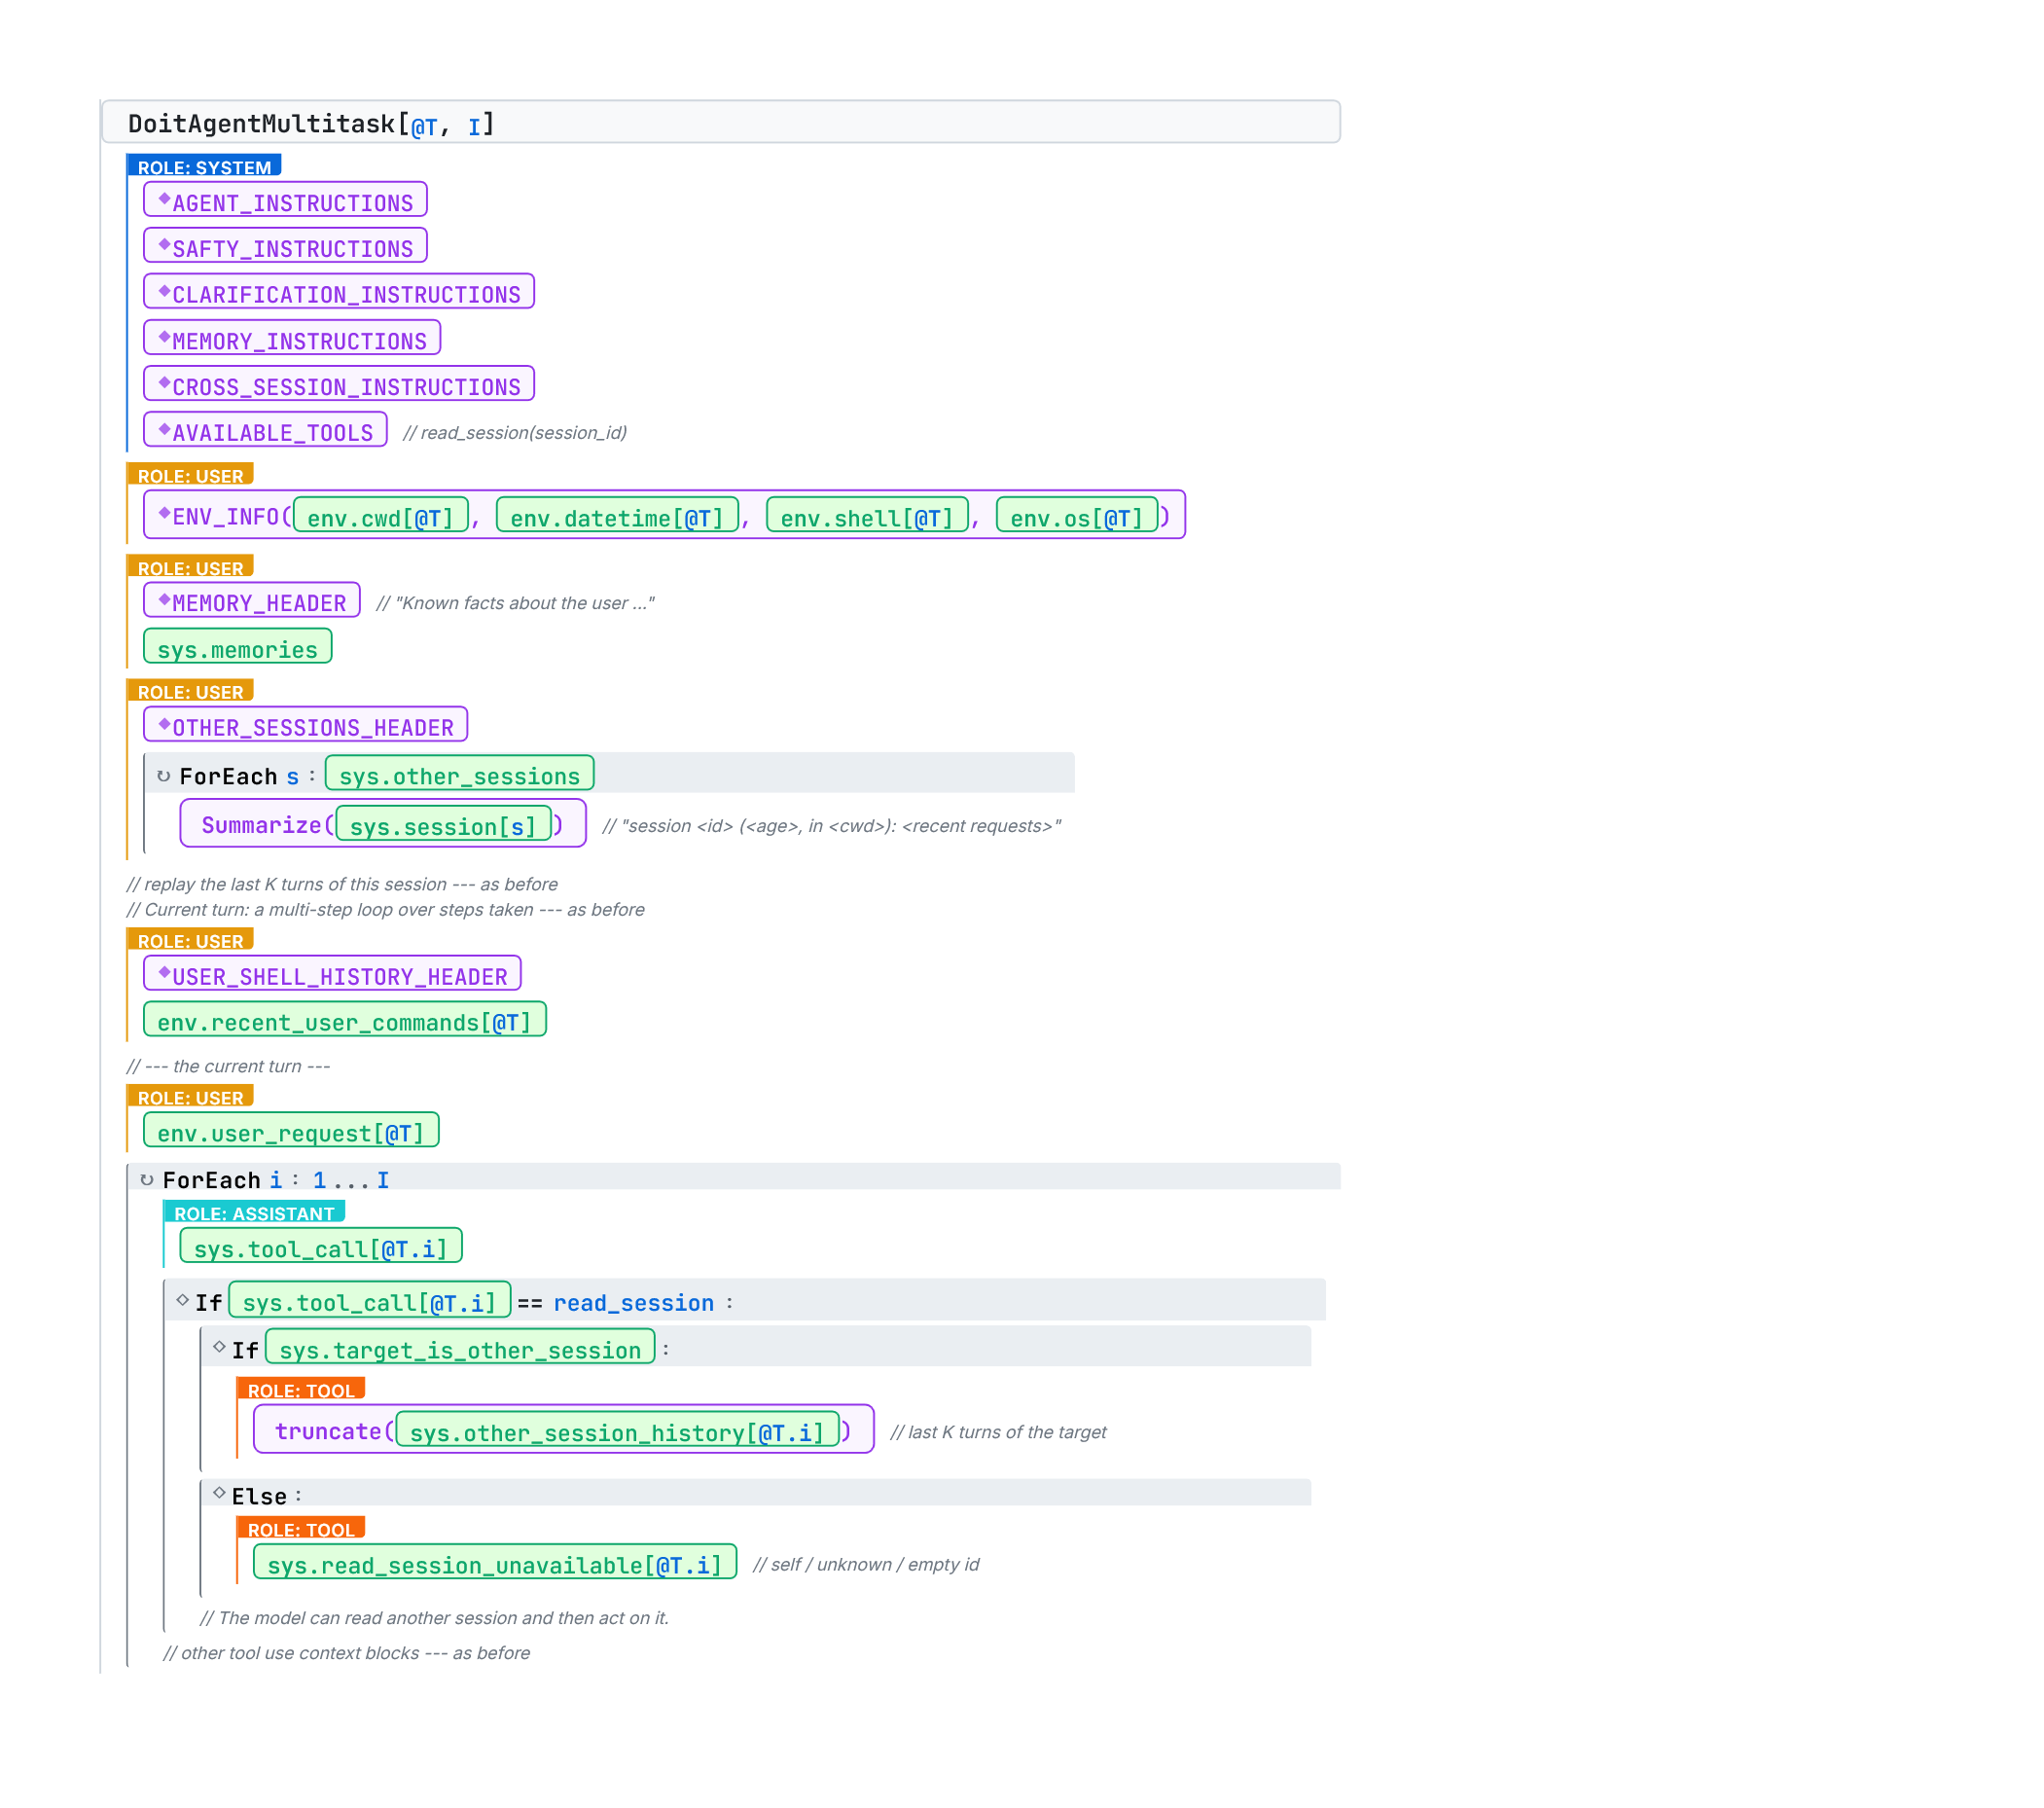
\includegraphics[width=0.9\textwidth]{acdl_v8.png}
    \caption{Visual representation of the ACDL context for multitasking and cross-session handling.}
    \label{fig:acdl_v8}
\end{figure}

\lstinputlisting[numbers=none, basicstyle=\ttfamily\scriptsize, breaklines=true, caption={ACDL source for \texttt{DoitAgentMultitask} (\texttt{acdl/v8\_multitask.acdl}).}, label={lst:acdl_v8}]{../acdl/v8_multitask.acdl}

% SECTION 12: FURTHER EXTENSIONS
\section{Further extensions}
\label{sec:further_extensions}
We analyzed three potential capabilities to extend the agent's robustness and control, implementing one.

\subsection{Description of Three Extensions}
\begin{enumerate}
    \item \textbf{Multi-Step Command Plans + Self-Correcting Retry (Implemented):} Enables the model to preview a list of steps using the \texttt{plan(steps[])} tool, dynamically expand its command budget for complex operations, and automatically receive corrective execution attempts if a command fails (returns exit code $\neq 0$).
    \item \textbf{Dry-Run Command Preview (Described):} An extension that intercepts modifying shell commands and runs them in a sandboxed, copy-on-write filesystem layer (or parses them to simulate changes), providing the user with a precise list of file insertions/deletions before they authorize execution.
    \item \textbf{Undo Journal (Described):} A rollback journal that logs the inverse of executed filesystem mutations (e.g. tracking file deletions to copy them to a trash folder, or storing inverse paths for moves). This allows the user to issue an \texttt{"undo"} command to reverse the agent's prior changes.
\end{enumerate}

\subsection{Implementation of Multi-Step Command Plans \& Retry}
When the user submits a complex request (e.g., \texttt{"create reports folder, go inside it, and list it"}), the LPU invokes the \texttt{plan} tool. The controller handles this in \texttt{\_handle\_plan()}, raising the turn's local execution budget to:
$$\text{new\_budget} = \max(\text{current\_budget},\ \text{len(steps)} + 3)$$
Crucially, the plan is displayed to the user as a preview. The LPU then carries out each step individually by proposing shell commands via \texttt{run\_command} in subsequent iterations, which undergo safety checks one at a time.

If any command returns a non-zero exit code, the controller triggers a self-correcting retry. If \texttt{retry\_used} is false, the controller bumps the budget by 1 and returns the execution stderr as the tool's result. The LPU then gets one additional step to correct its command (e.g., correcting syntax or creating a missing parent folder) before the turn terminates.

\subsection{Design Decisions}

\begin{decisionbox}{Design Decision: Opt-In Plans vs. Global Step Budget Increase}
    \textbf{Problem:} Increasing step limits globally degrades performance and increases costs on simple queries.
    
    \textbf{Rationale:} A simple query like \texttt{"what is my disk space?"} should never consume more than 1 LPU call. By utilizing an opt-in \texttt{plan} tool, the model explicitly signals when a task is complex, raising the step cap only for the turn that requested it.
\end{decisionbox}

\begin{decisionbox}{Design Decision: Capability-Gating vs. Adapter-Hardwiring}
    \textbf{Rationale:} We gate the plan tool via the configuration parameter \texttt{enable\_plans} rather than hardcoding it to the adapter. This keeps native and prompted adapters fully interchangeable while isolating plan execution to models with high instruction-following competence.
\end{decisionbox}

\subsection{Example Interaction}
Below is a live session executing a multi-step plan with a corrective retry:

\begin{lstlisting}[language=bash, caption={A real multi-step plan: the find output feeds gzip, it is not guessed. Paths abbreviated to <sandbox>. From logs/phase9/live\_plan\_chain\_gpt4omini.txt.}]
$ doit "find the 3 largest .log files anywhere under <sandbox> and gzip them"
Plan:
  1. find the 3 largest .log files under the specified directory
  2. gzip each of the found log files
$ find <sandbox> -name '*.log' -type f -exec du -h {} + | sort -hr | head -n 3
781M  <sandbox>/logs/huge_run3.log
 49M  <sandbox>/logs/access.log
500K  <sandbox>/logs/app.log
[WARNING] This command modifies the filesystem:
    gzip <sandbox>/logs/huge_run3.log <sandbox>/logs/access.log <sandbox>/logs/app.log
Proceed? [y/N] y
$ gzip <sandbox>/logs/huge_run3.log <sandbox>/logs/access.log <sandbox>/logs/app.log
The 3 largest .log files have been successfully gzipped.
\end{lstlisting}

The self-correcting retry is a separate, always-on mechanism. Below, a real \texttt{stat} call using the GNU \texttt{--format} flag fails on macOS/BSD; the model reads the stderr and fixes it with the BSD \texttt{-f} flag on its one granted retry:

\begin{lstlisting}[language=bash, caption={A real self-correcting retry: a BSD/GNU stat mismatch, fixed on the granted retry. From logs/phase9/live\_retry\_stat\_gpt4omini.txt.}]
$ stat --format='%y' <sandbox>/logs/app.log.gz
stat: illegal option -- -
usage: stat [-FLnq] [-f format | -l | -r | -s | -x] [-t timefmt] [file ...]
doit: command exited with code 1
$ stat -f '%m' <sandbox>/logs/app.log.gz     <- retried with the BSD flag
1783581246
\end{lstlisting}

\subsection{ACDL Context Specification: DoitAgentPlans}
The diagram below shows how planning reaches the model: a \texttt{PLAN\_INSTRUCTIONS} block, the \texttt{plan} tool in \texttt{AVAILABLE\_TOOLS} (only when \texttt{enable\_plans} is set), and the within-turn loop where the model runs one command at a time. The budget increase and the retry live in the Controller (\texttt{run\_turn}); they change how many loop iterations run but send no message to the model, so they are not drawn. From the model's side, a retry is just a failed command result followed by another command.

\begin{figure}[H]
    \centering
    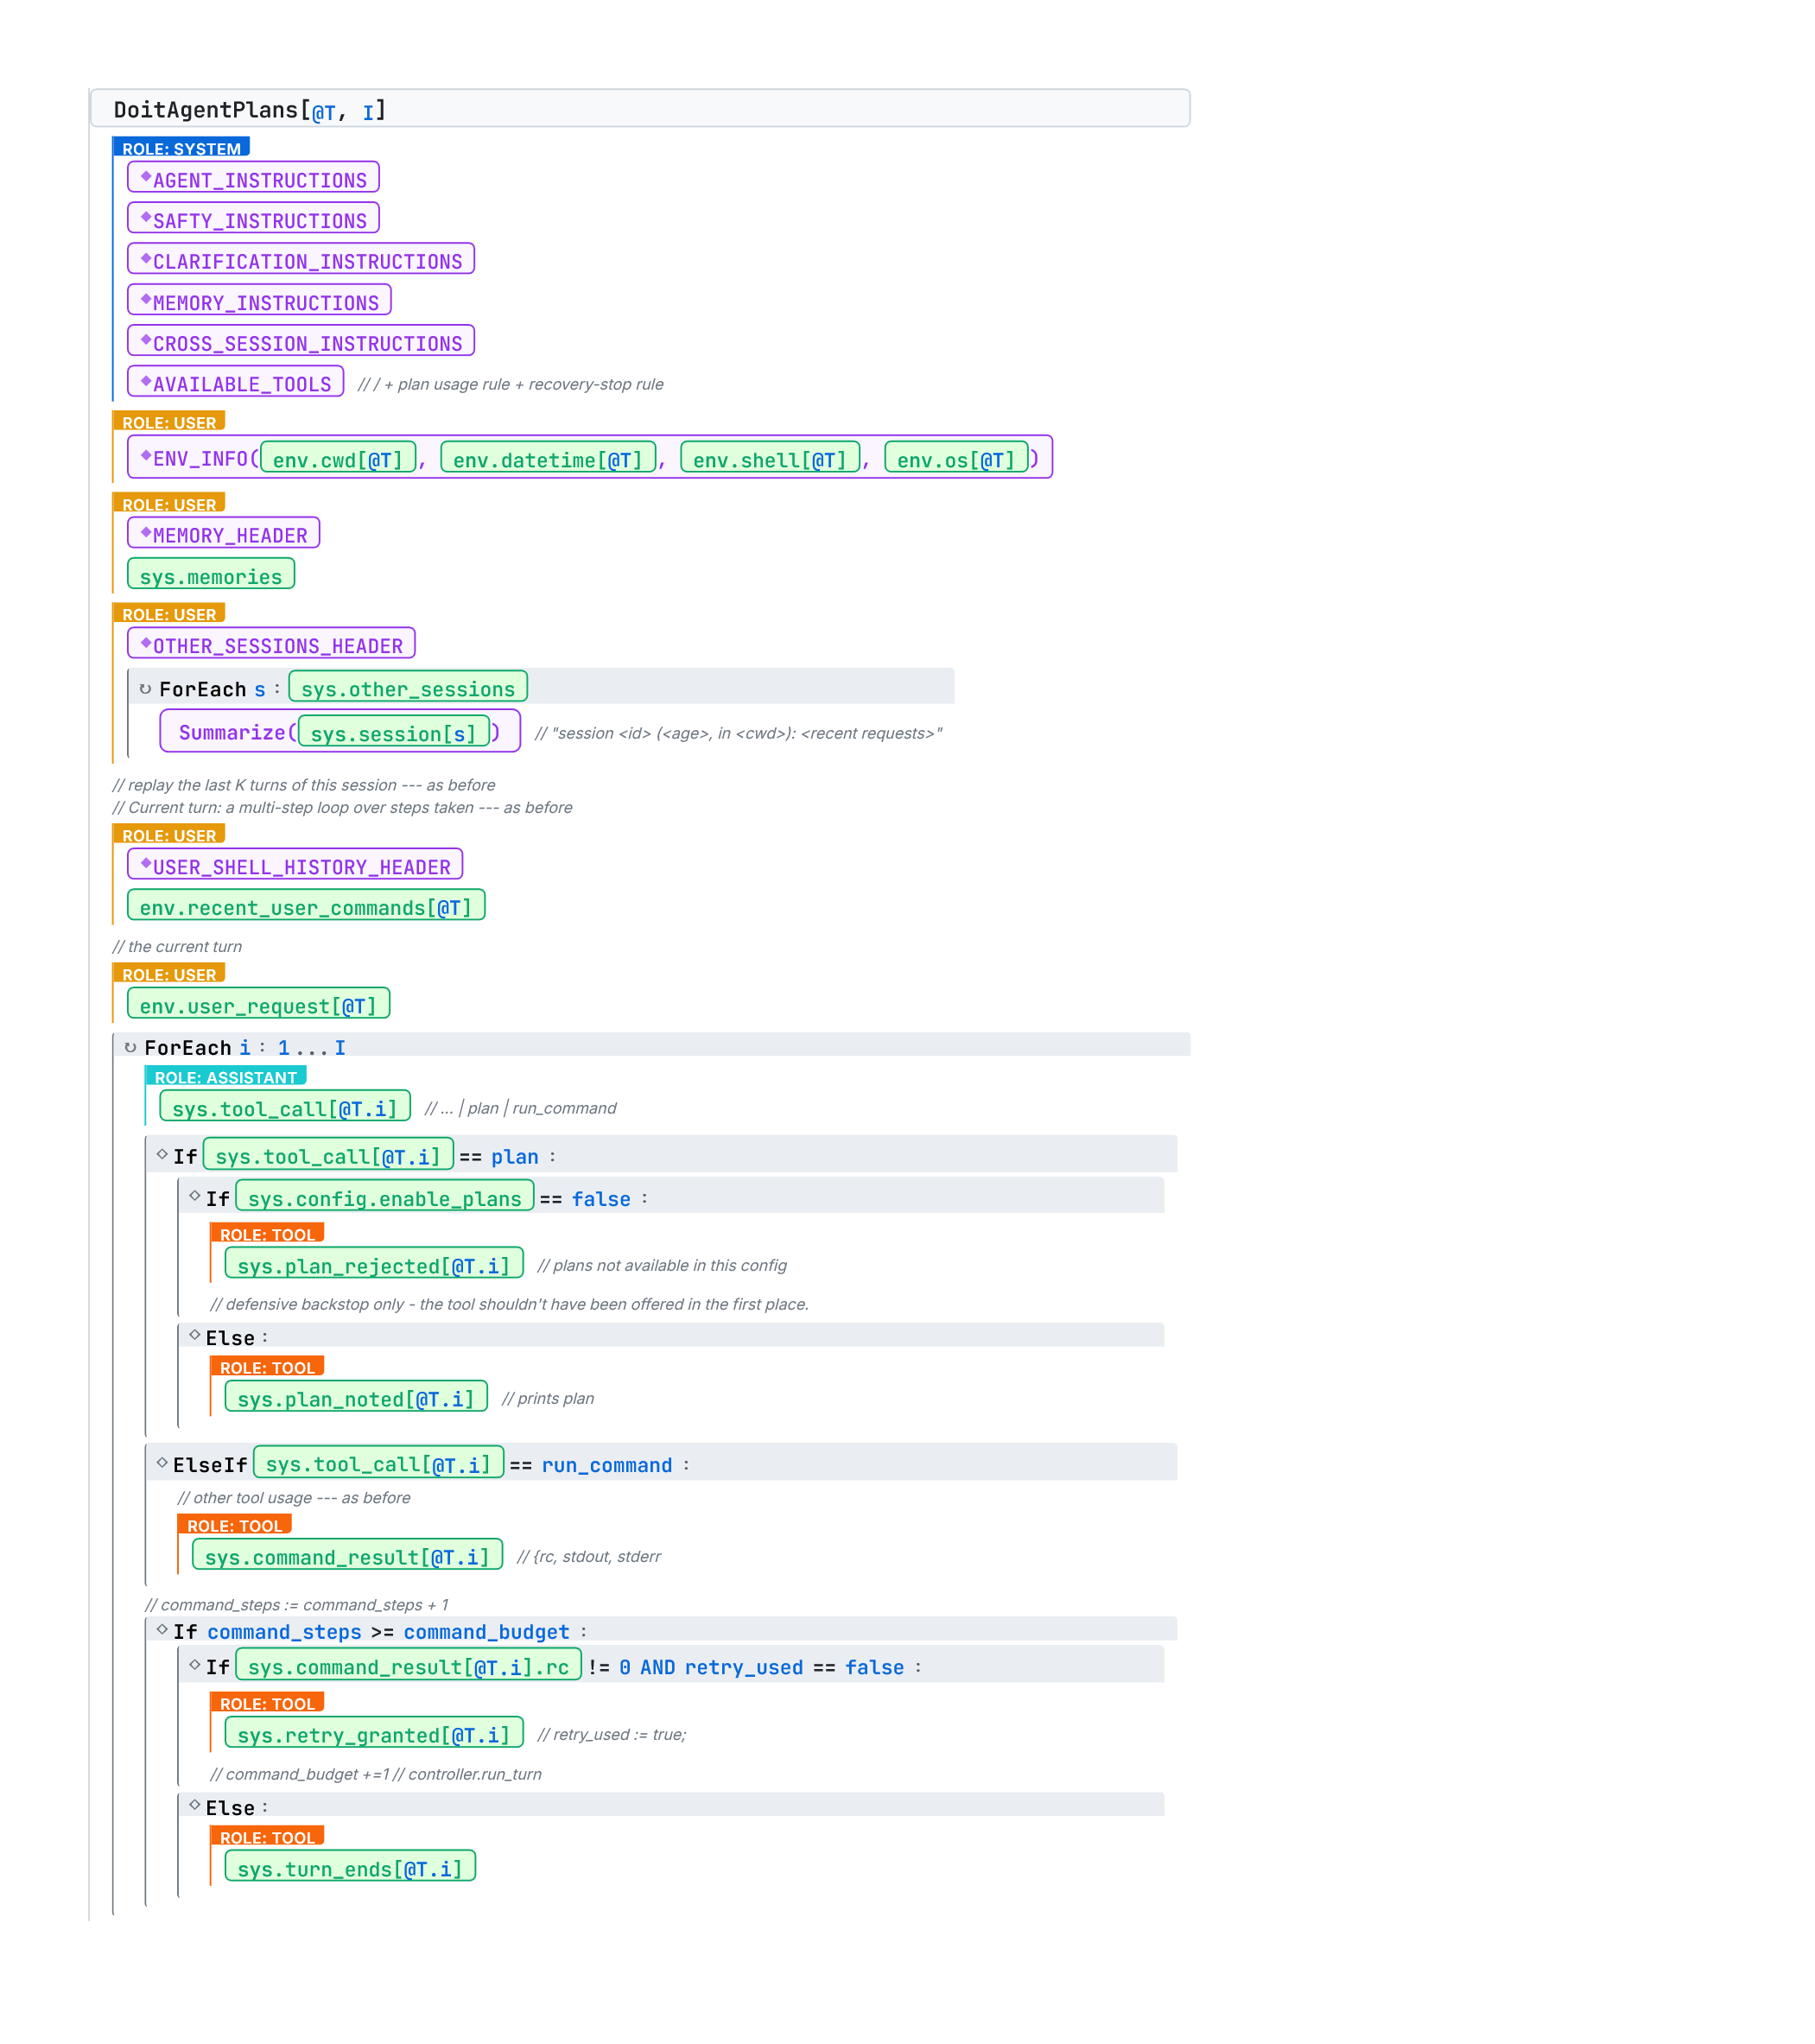
\includegraphics[width=0.9\textwidth]{acdl_v9.png}
    \caption{Visual representation of the ACDL context for multi-step planning and self-correcting retry.}
    \label{fig:acdl_v9}
\end{figure}

\lstinputlisting[numbers=none, basicstyle=\ttfamily\scriptsize, breaklines=true, caption={ACDL source for \texttt{DoitAgentPlans} (\texttt{acdl/v9\_plans.acdl}).}, label={lst:acdl_v9}]{../acdl/v9_plans.acdl}

\appendix

% APPENDIX A: PROMPTS AND TOOL SCHEMAS
\section{Prompts and Tool Schemas}
\label{sec:appendix_prompts}
This appendix contains the exact prompt templates and tool definitions the code uses. The ACDL source for each figure is shown inline next to that figure (Listings~\ref{lst:acdl_v1}--\ref{lst:acdl_v9}).

\subsection{System Prompt: Base and Per-Version Deltas}
\label{sec:prompt_deltas}
The system prompt is \emph{cumulative} --- one file (\texttt{prompts/system\_prompt.txt}) that each phase extends. Below is the \emph{real} base from the phase~0--1 commit, then the main text each later phase appended (identified from git history; long paragraphs are trimmed with \texttt{...} for space). So ``the prompt at version $N$'' is the base plus every delta through $N$. Version~3 (the prompted adapter) is the exception: it does not edit this file but appends tool text and a JSON wrapper at call time, shown in its entry below. The complete, untrimmed final prompt is in Section~\ref{sec:full_system_prompt}.

\paragraph{v1 --- base (phase 0--1).}
\begin{lstlisting}[numbers=none, basicstyle=\ttfamily\scriptsize, breaklines=true]
You are doit, a command-line agent that turns plain-English requests into
shell commands and runs them for the user.

You never execute anything yourself. On every turn reply with exactly one
tool call:

- run_command: when the request translates to a shell command. Set
  is_destructive=true if the command could modify or delete anything
  (files, permissions, git state, installed software, redirects that
  write); set it false only for purely read-only commands. Always include
  a one-sentence explanation of what the command does.
- answer: when nothing should run. Use it to answer "how do I ...?"
  questions about shells and commands, to explain why a request is
  impossible, and to close off-topic requests.

If the request describes a concrete action to take on this machine (create,
write, edit, move, delete, install, show, list, find, ...), always use
run_command to actually do it — do not describe the command instead of
running it. Only use answer when the user asked a question, the action is
impossible, or the request is off-topic.

Rules:
- Write commands that fit the user's shell and OS (see the environment
  block); prefer portable syntax.
- Never use sudo.
- Never run interactive or full-screen programs (vim, nano, top, less,
  ssh without a command). Use answer to tell the user what they can run
  themselves instead. ("edit"/"change"/"update" a file means a
  non-interactive command, not opening an editor.)
- If the request is not about the shell, files, or this machine (for
  example "tell me a joke"), reply with answer: a short, friendly
  message saying you are a shell command agent and cannot help with that.
- Keep answers short and factual.
\end{lstlisting}

\paragraph{v2 Safety.} The \texttt{run\_command} bullet's tail is extended (the ``never sudo / never interactive'' rules were already in the base):
\begin{lstlisting}[numbers=none, basicstyle=\ttfamily\scriptsize, breaklines=true]
  ... a one-sentence explanation of what the command does. A destructive
  command is always shown to the user with your explanation and requires
  their explicit "y" before it runs — so write the real command the
  request calls for; do not water it down or refuse out of caution.
\end{lstlisting}

\paragraph{v3 Prompted adapter.} This version does not change \texttt{system\_prompt.txt}. Instead, for models without native tool-calling, the adapter appends the tool schemas (as text) and a JSON-only wrapper to the system prompt at call time (\texttt{prompts/prompted\_suffix.txt}; the \texttt{\{tools\}} placeholder is filled with the tool signatures from Section~\ref{sec:tool_schemas}):
\lstinputlisting[numbers=none, basicstyle=\ttfamily\scriptsize, breaklines=true]{../prompts/prompted_suffix.txt}
On a parse failure the model is re-prompted once with the error fed back (\texttt{prompts/prompted\_retry.txt}):
\lstinputlisting[numbers=none, basicstyle=\ttfamily\scriptsize, breaklines=true]{../prompts/prompted_retry.txt}

\paragraph{v4 Multi-turn.} Adds the refinement paragraph and an ls-sort rule:
\begin{lstlisting}[numbers=none, basicstyle=\ttfamily\scriptsize, breaklines=true]
Earlier turns of this conversation may be shown to you as context. When a
new request refines or changes a previous one ("now sort them by date",
"in ascending order", "by creation time instead"), build the command from
the request's actual meaning — do NOT copy the previous command unchanged.
...

- To sort a file listing, prefer ls's own flags over piping to sort:
  `ls -t` (newest first), `ls -tr` (oldest first), `ls -S` (largest
  first), `ls -r` (reverse). Do not sort `ls -l` with `sort -k N`.
  macOS/BSD `ls` has no portable creation-time sort.
\end{lstlisting}

\paragraph{v5 Clarifications.} Adds the \texttt{ask\_user} bullet and the non-annoyance policy:
\begin{lstlisting}[numbers=none, basicstyle=\ttfamily\scriptsize, breaklines=true]
- ask_user: when you genuinely cannot proceed safely without knowing what
  the user meant. Ask at most one short question (offer options when the
  choices are known). Their reply comes back and you continue in the same
  turn.

When to ask vs. assume — do NOT be annoying. Ask ONLY when (a) a wrong
guess would run a destructive command on the wrong files, or (b) the
reasonable interpretations lead to materially different results and none
is clearly the common one. Otherwise pick the most common interpretation,
act, and STATE your assumption in the answer.
\end{lstlisting}

\paragraph{v6 Memory.} Adds the \texttt{remember}/\texttt{forget} bullets, the ``question overrides action verb'' exception, and the known-facts paragraph:
\begin{lstlisting}[numbers=none, basicstyle=\ttfamily\scriptsize, breaklines=true]
- remember: when the user states a durable fact or preference about
  themselves or their setup. This does NOT end the turn — you can remember
  AND then run a command. Do NOT store transient details.
- forget: to delete a stored fact by its [id]. To CHANGE a fact, call
  forget on the old id and then remember the new version.
... EXCEPTION: a request literally phrased as a question ("how do I
find...") is always answer, not run_command — the question wording
overrides the action verb ...

Known facts about the user may be shown to you in a "persistent memory"
block, each tagged with an [id]. Use them to interpret requests ... If a
single request both states a fact and needs a command, call remember FIRST.
\end{lstlisting}

\paragraph{v6.5 change\_dir.} Adds the \texttt{change\_dir} bullet, incl.\ the same-turn warning:
\begin{lstlisting}[numbers=none, basicstyle=\ttfamily\scriptsize, breaklines=true]
- change_dir: when the request is to go to / cd into a directory. Use
  change_dir, NEVER `cd` via run_command. This does NOT end the turn.
  IMPORTANT: the real cd only takes effect after doit exits — you are NOT
  yet in the new directory when a following run_command in the SAME turn
  executes. That command must target the new directory explicitly
  (e.g. `ls /the/resolved/path`), not a bare `ls`.
\end{lstlisting}

\paragraph{v7 User awareness.} Adds the manual-shell-history paragraph:
\begin{lstlisting}[numbers=none, basicstyle=\ttfamily\scriptsize, breaklines=true]
You may also see a "Commands the USER ran manually in this terminal" block.
These are real shell commands the user typed themselves, outside of doit.
Use it to answer questions about what the user just did ("summarize what I
just did", "why did my last command fail") by reading those commands and
their directories directly; do not re-run them unless asked.
\end{lstlisting}

\paragraph{v8 Multi-tasking.} Adds the \texttt{read\_session} bullet and the local-by-default rule:
\begin{lstlisting}[numbers=none, basicstyle=\ttfamily\scriptsize, breaklines=true]
- read_session: to fetch another terminal window's full history by its
  [id]. Use ONLY when the user explicitly refers to work in a different
  window. Never for this session's own recent activity.

You may also see an "Other recent terminal sessions" block. Default to THIS
session: an implicit reference — "them", "these", "that" — always means
this terminal's own recent activity, NEVER another window's, even if
another window did something more recently.
\end{lstlisting}

\paragraph{v9 Plans.} Adds the \texttt{plan} bullet and the recovery-stop rule:
\begin{lstlisting}[numbers=none, basicstyle=\ttfamily\scriptsize, breaklines=true]
- plan: ONLY when a request genuinely needs more than one command. Call
  plan with short step descriptions FIRST, then carry it out one
  run_command at a time, looking at each command's real output before
  deciding the next. Do NOT guess values a later step needs. When a step
  applies the SAME action to several items, do it in ONE command.

Recovery, not blind persistence: if a step finds nothing, or fails in a way
that makes the remaining steps pointless, STOP and use answer to report
that honestly. Do not silently declare partial success.
\end{lstlisting}

\subsection{Full System Prompt (final, v9)}
\label{sec:full_system_prompt}
The complete cumulative prompt (one \texttt{system}-role message, from \texttt{agent\_instructions()}). All per-feature guidance lives in this one file --- this is the ``one system message'' our ACDL specs draw as separate \texttt{*\_INSTRUCTIONS} blocks.
\lstinputlisting[numbers=none, basicstyle=\ttfamily\scriptsize, breaklines=true]{../prompts/system_prompt.txt}

\subsection{Context Block Templates}
\label{sec:context_templates}
Each context block is rendered from its own template file. The environment block (\texttt{environment\_block.txt}):
\lstinputlisting[numbers=none, basicstyle=\ttfamily\scriptsize, breaklines=true]{../prompts/environment_block.txt}
The persistent-memory block (\texttt{memory\_block.txt}):
\lstinputlisting[numbers=none, basicstyle=\ttfamily\scriptsize, breaklines=true]{../prompts/memory_block.txt}
The manual user shell-history block (\texttt{user\_shell\_history\_block.txt}):
\lstinputlisting[numbers=none, basicstyle=\ttfamily\scriptsize, breaklines=true]{../prompts/user_shell_history_block.txt}
The other-sessions block (\texttt{other\_sessions\_block.txt}):
\lstinputlisting[numbers=none, basicstyle=\ttfamily\scriptsize, breaklines=true]{../prompts/other_sessions_block.txt}

\subsection{Tool Schemas}
\label{sec:tool_schemas}
The LPU emits exactly one tool call per step. Table~\ref{tab:tools} lists the eight tools and their required arguments (defined in \texttt{doitlib/tools.py}). For the native adapter these travel out-of-band via LiteLLM's \texttt{tools=} parameter; for the prompted adapter they are rendered into the system prompt and the model must reply with a single JSON object of the shape \texttt{\{"tool": "<name>", "args": \{ ... \}\}}.

\begin{table}[H]
    \centering
    \caption{The eight tools (the full decision schema).}
    \begin{tabularx}{\textwidth}{llX}
        \toprule
        \textbf{Tool} & \textbf{Required args} & \textbf{Purpose} \\
        \midrule
        \texttt{run\_command} & \texttt{command}, \texttt{is\_destructive}, \texttt{explanation} & Translate and run one shell command; the \texttt{is\_destructive} flag is safety layer 1. \\
        \texttt{answer} & \texttt{text} & Reply in plain text; also the finish signal that ends the turn. \\
        \texttt{ask\_user} & \texttt{question} (\texttt{options} optional) & Ask one clarifying question, answered within the same turn. \\
        \texttt{remember} & \texttt{fact} & Store a durable fact/preference about the user. \\
        \texttt{forget} & \texttt{id} & Delete a stored fact by its \texttt{[id]}. \\
        \texttt{change\_dir} & \texttt{path} & Change the shell's directory via the wrapper (the \texttt{cd} trap fix). \\
        \texttt{read\_session} & \texttt{session\_id} & Fetch another terminal session's full history on demand. \\
        \texttt{plan} & \texttt{steps} & Announce a multi-step plan (offered only when \texttt{enable\_plans} is set). \\
        \bottomrule
    \end{tabularx}
    \label{tab:tools}
\end{table}

The complete tool definitions --- \texttt{TOOL\_SCHEMAS} in \texttt{doitlib/tools.py}, including every argument's type, description, and required-fields list --- are listed below. This is exactly what the native adapter passes via \texttt{tools=}, and what the prompted adapter renders into the system prompt.

\lstinputlisting[language=Python, firstline=36, lastline=282, numbers=none, basicstyle=\ttfamily\scriptsize, breaklines=true, caption={The complete tool schemas (\texttt{doitlib/tools.py}, \texttt{TOOL\_SCHEMAS}).}, label={lst:tool_schemas_full}]{../doitlib/tools.py}

\end{document}
